
	\subsection{Figures}
	Figures \ref{fig:coveragemap1} - \ref{fig:coveragemap18} show the frequency with which the true value of the parameter $\beta_1$ was covered by the 95\% confidence intervals at each location under each simulation setting. The left column shows the coverage frequency of the 95\% CI of the GAL using the unshrunk-bootstrap method of CI construction. The middle column is the coverage frequency of the 95\% CI the O-GWR using the bootstrap to generate the CI. The right column is the relative efficiency of the GAL to O-GWR. In the first two columns, the color white is used to indicate areas where the nominal coverage frequency of 95\% is achieved, while blue codes areas that exceeded 95\% coverage and orange codes areas that fell short of 95\% coverage. In the third column, the color white indicates areas where the relative efficiency is unity, while orange indicates areas where the relative efficiency was less than unity and blue indicates areas where the relative efficiency exceeded unity.\\	
	
	
	\begin{center}
		%\centering
		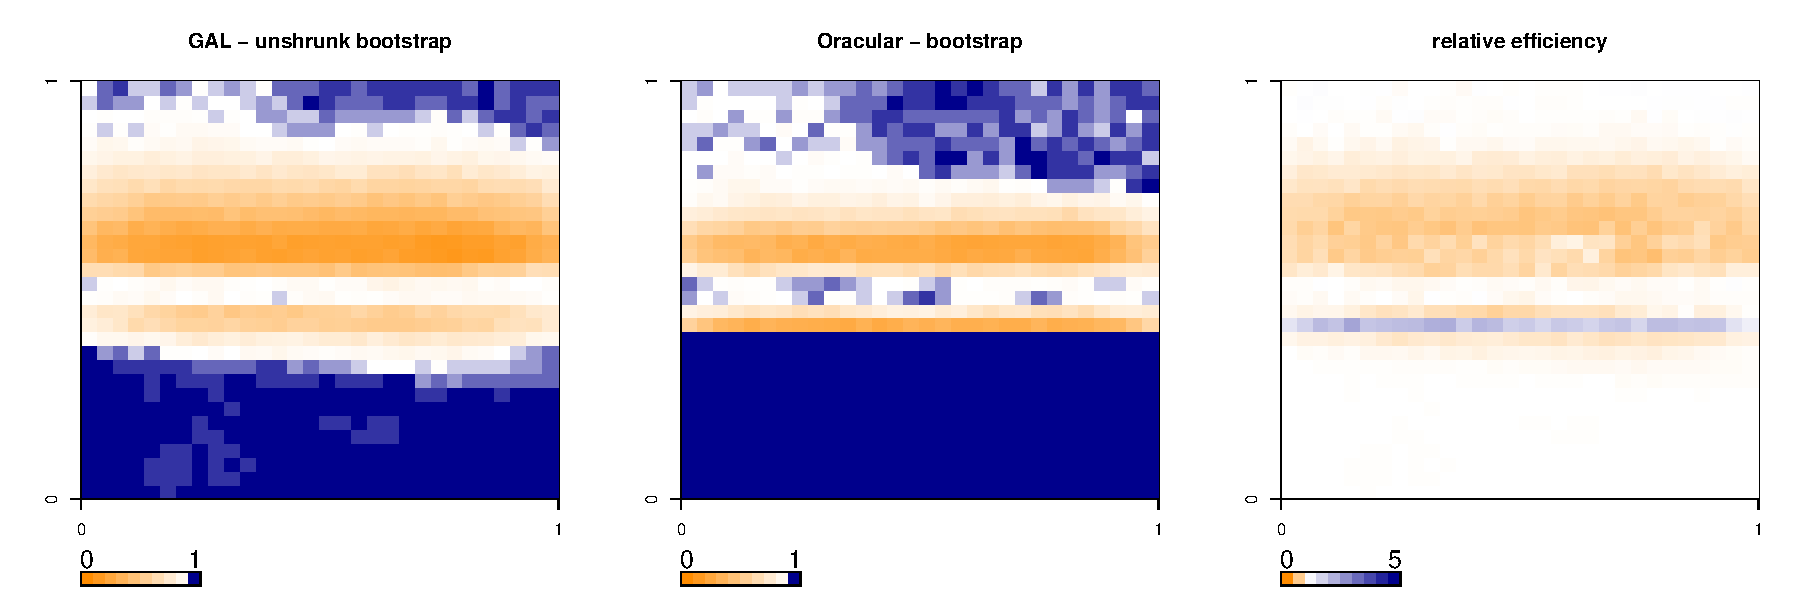
\includegraphics[width=0.99\textwidth]{../../figures/X1-28-1.pdf}
		%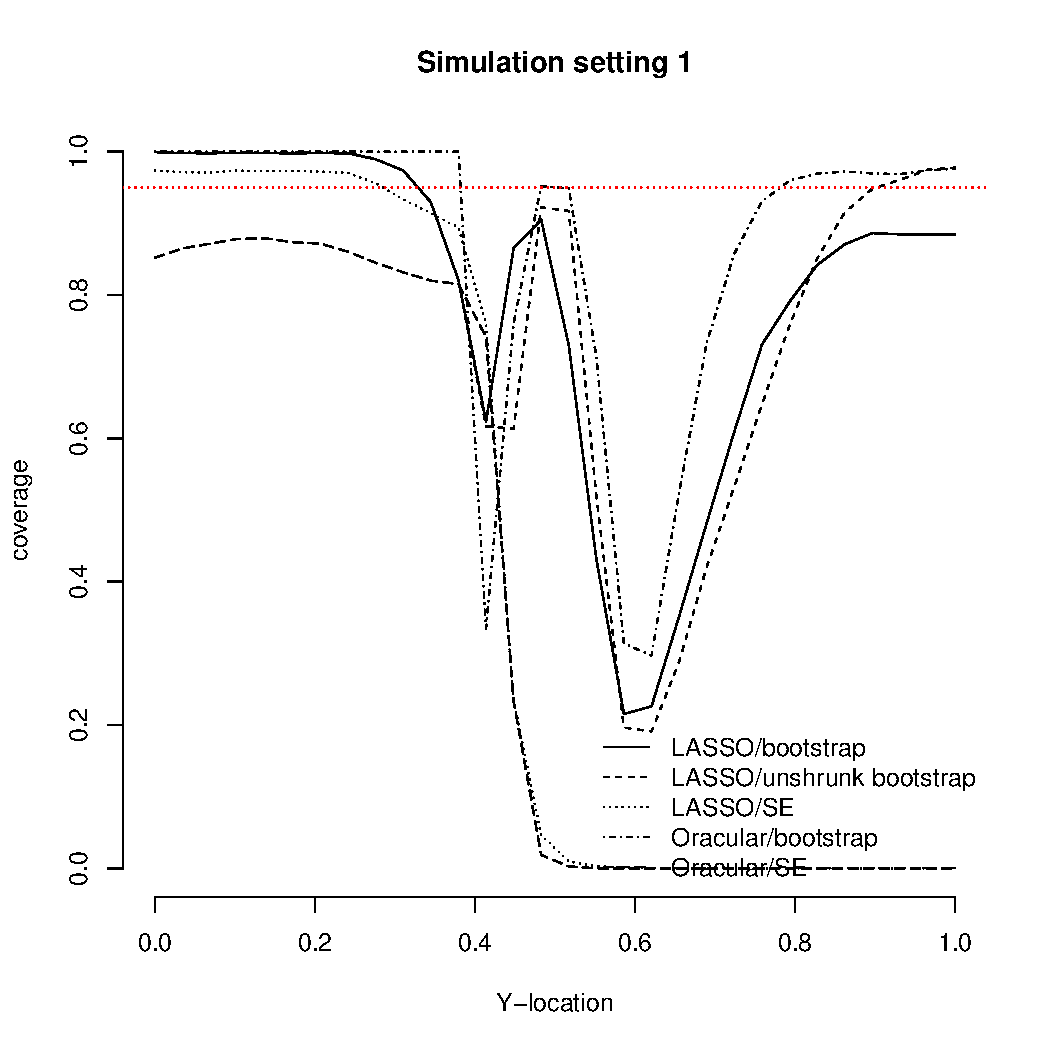
\includegraphics[width=\textwidth]{../../figures/simulation/28-1-profile-coverage.pdf}
		\captionof{figure}{Coverage frequency of 95\% CIs: setting 1\label{fig:coveragemap1}}
	\end{center}
        
	\begin{center}
		%\centering
		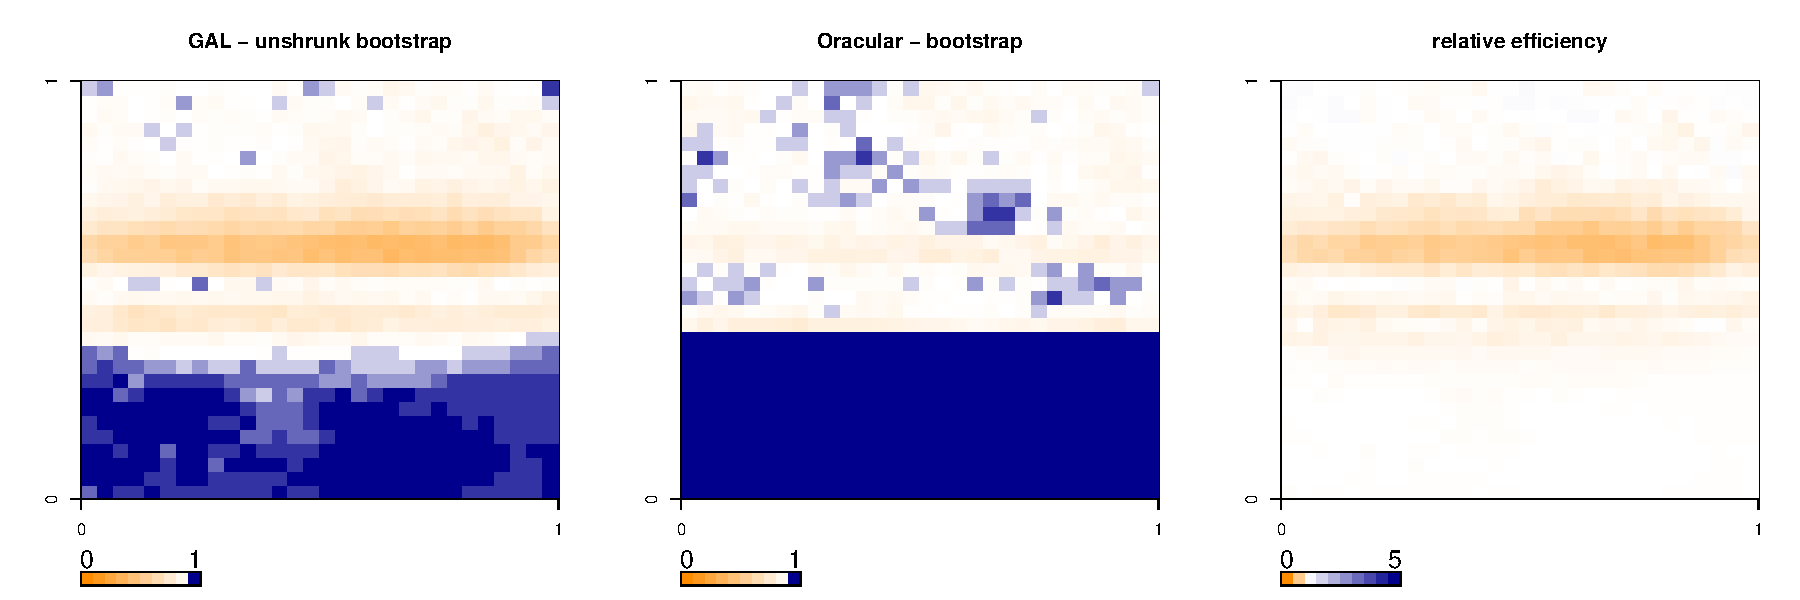
\includegraphics[width=0.99\textwidth]{../../figures/X1-28-2.pdf}
		%\includegraphics[width=\textwidth]{../../figures/simulation/28-2-profile-coverage.pdf}
		\captionof{figure}{Coverage frequency of 95\% CIs: setting 2\label{fig:coveragemap2}}
	\end{center}
	
	\begin{center}
		%\centering
		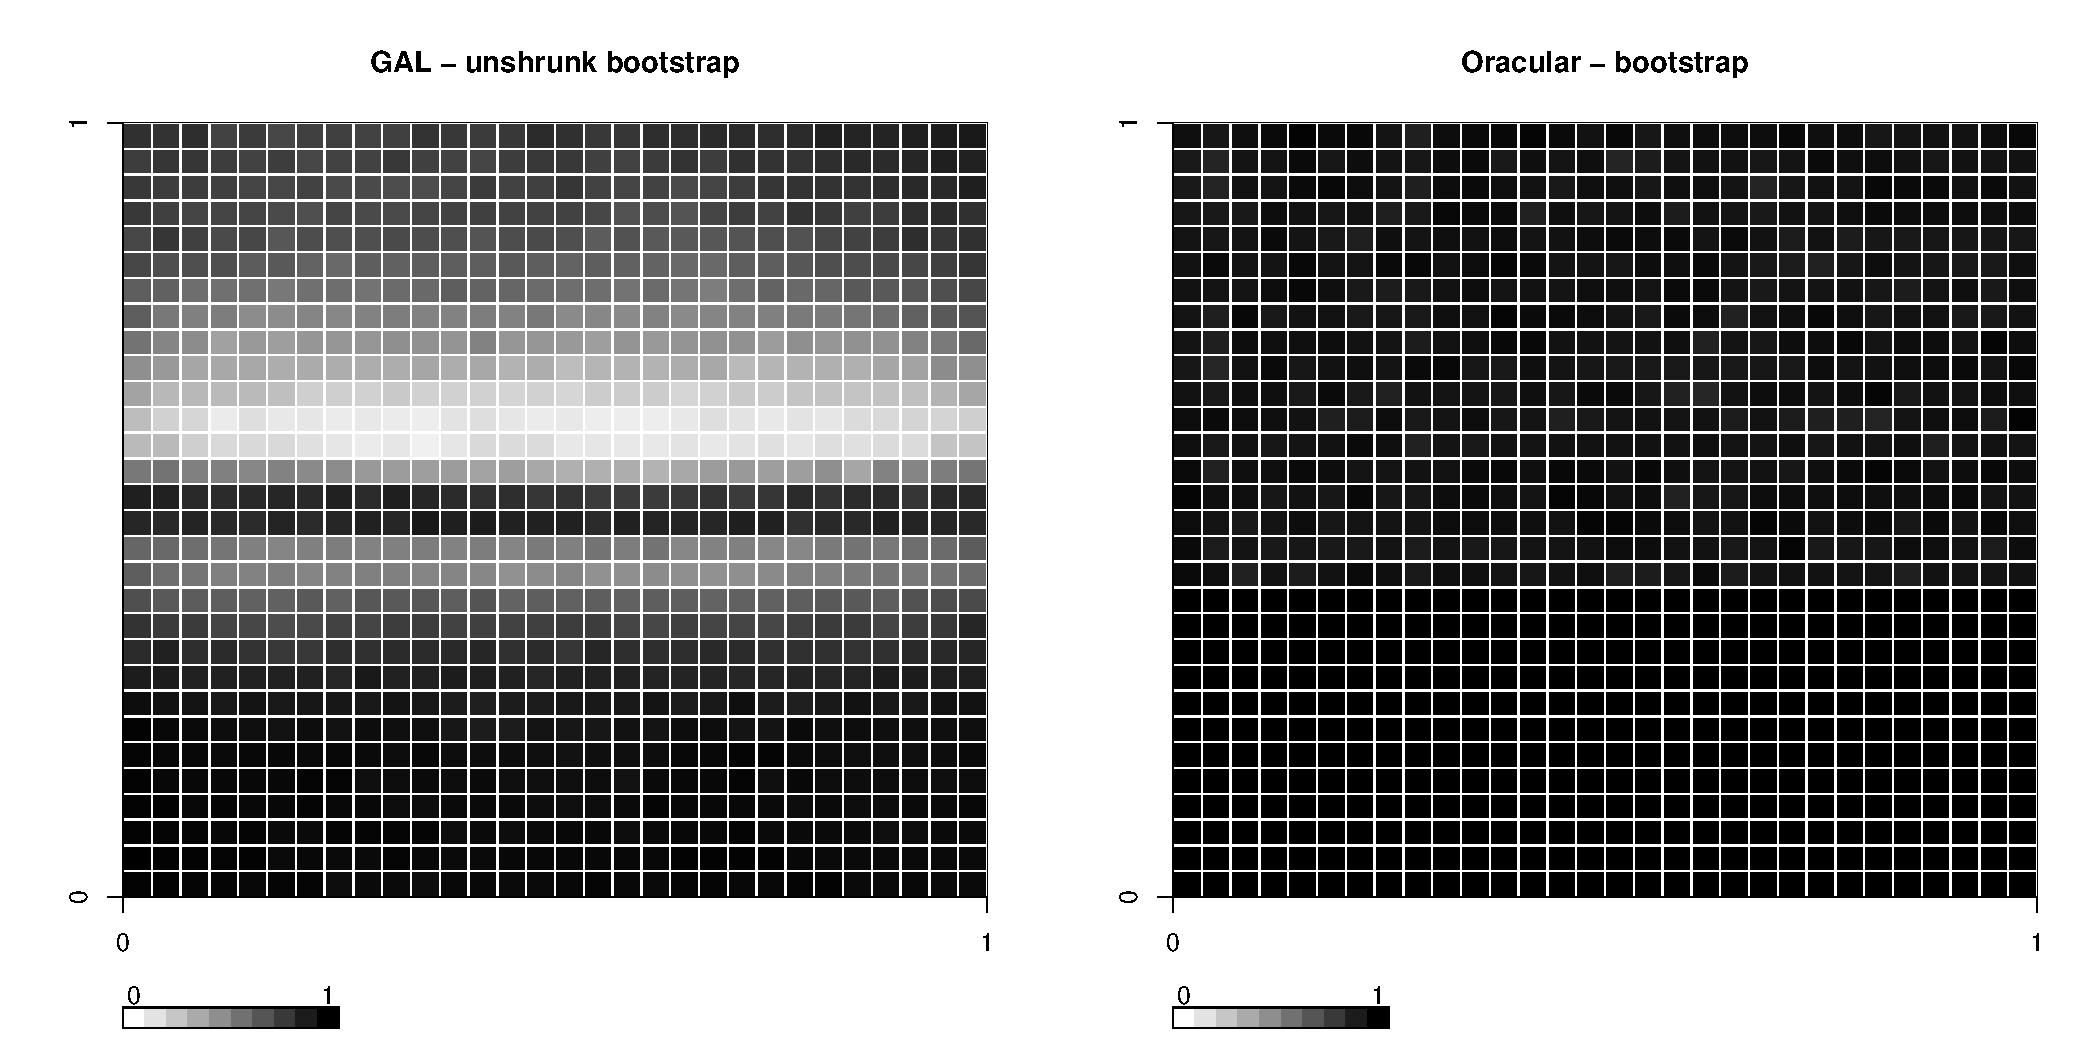
\includegraphics[width=0.99\textwidth]{../../figures/X1-28-3.pdf}
		%\includegraphics[width=\textwidth]{../../figures/simulation/28-3-profile-coverage.pdf}
		\captionof{figure}{Coverage frequency of 95\% CIs: setting 3\label{fig:coveragemap3}}
	\end{center}
	
	\begin{center}
		%\centering
		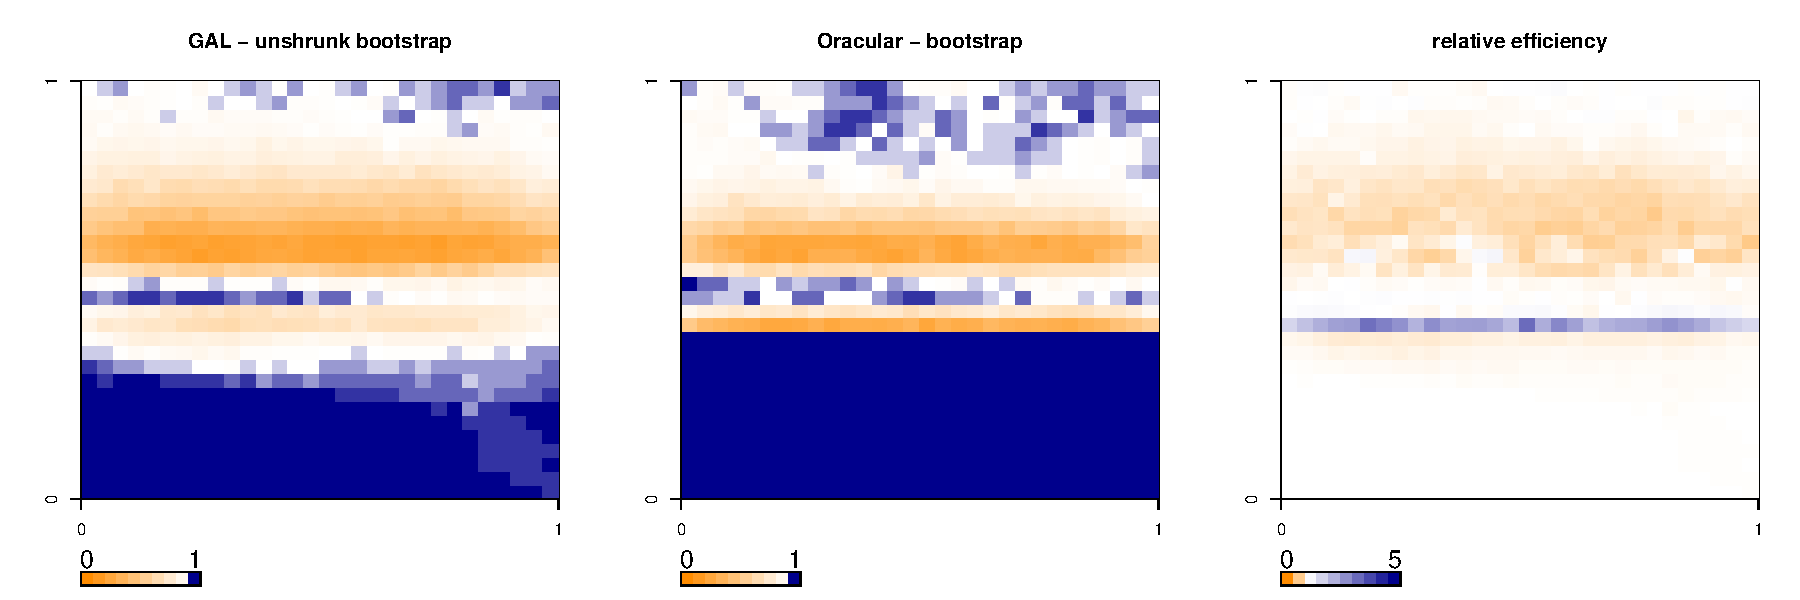
\includegraphics[width=0.99\textwidth]{../../figures/X1-28-4.pdf}
		%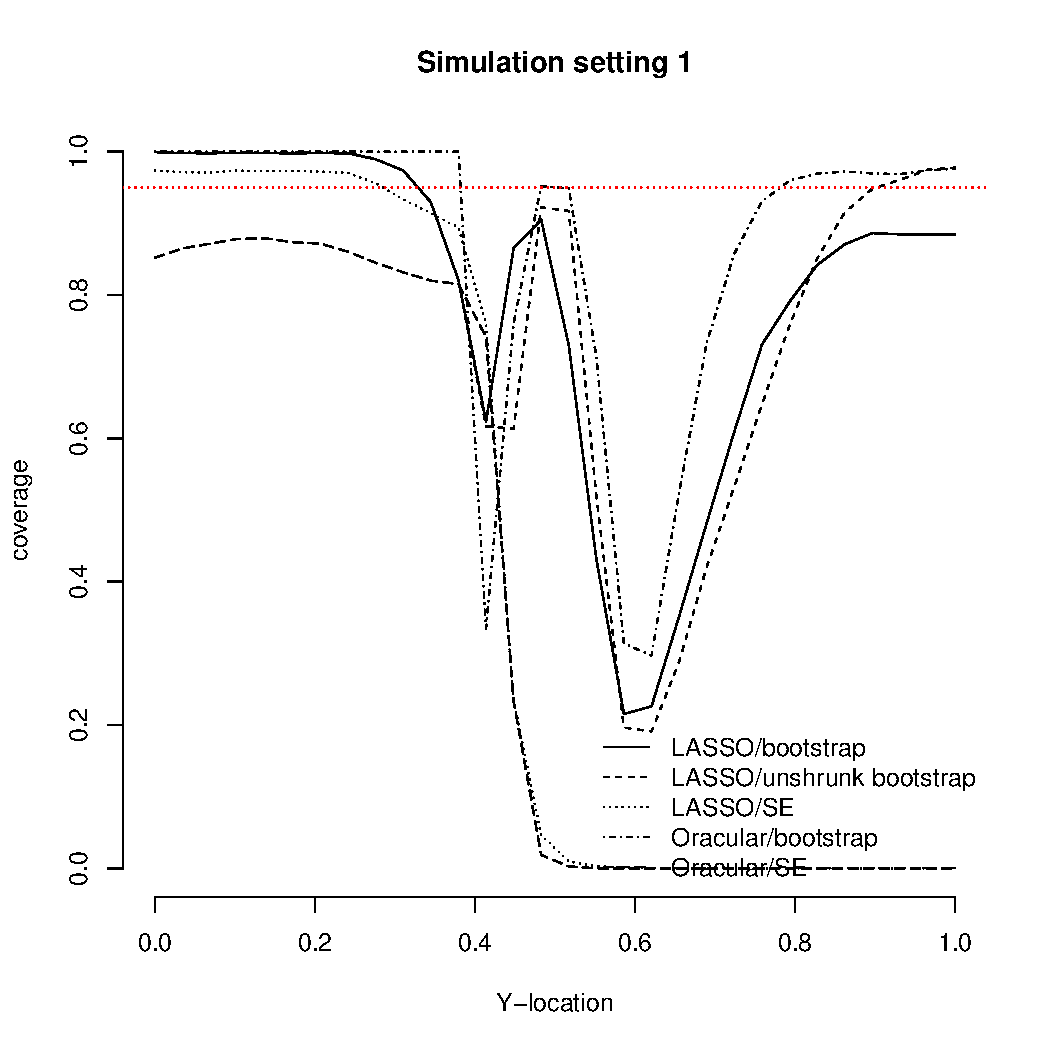
\includegraphics[width=\textwidth]{../../figures/simulation/28-1-profile-coverage.pdf}
		\captionof{figure}{Coverage frequency of 95\% CIs: setting 4\label{fig:coveragemap4}}
	\end{center}
        
	\begin{center}
		%\centering
		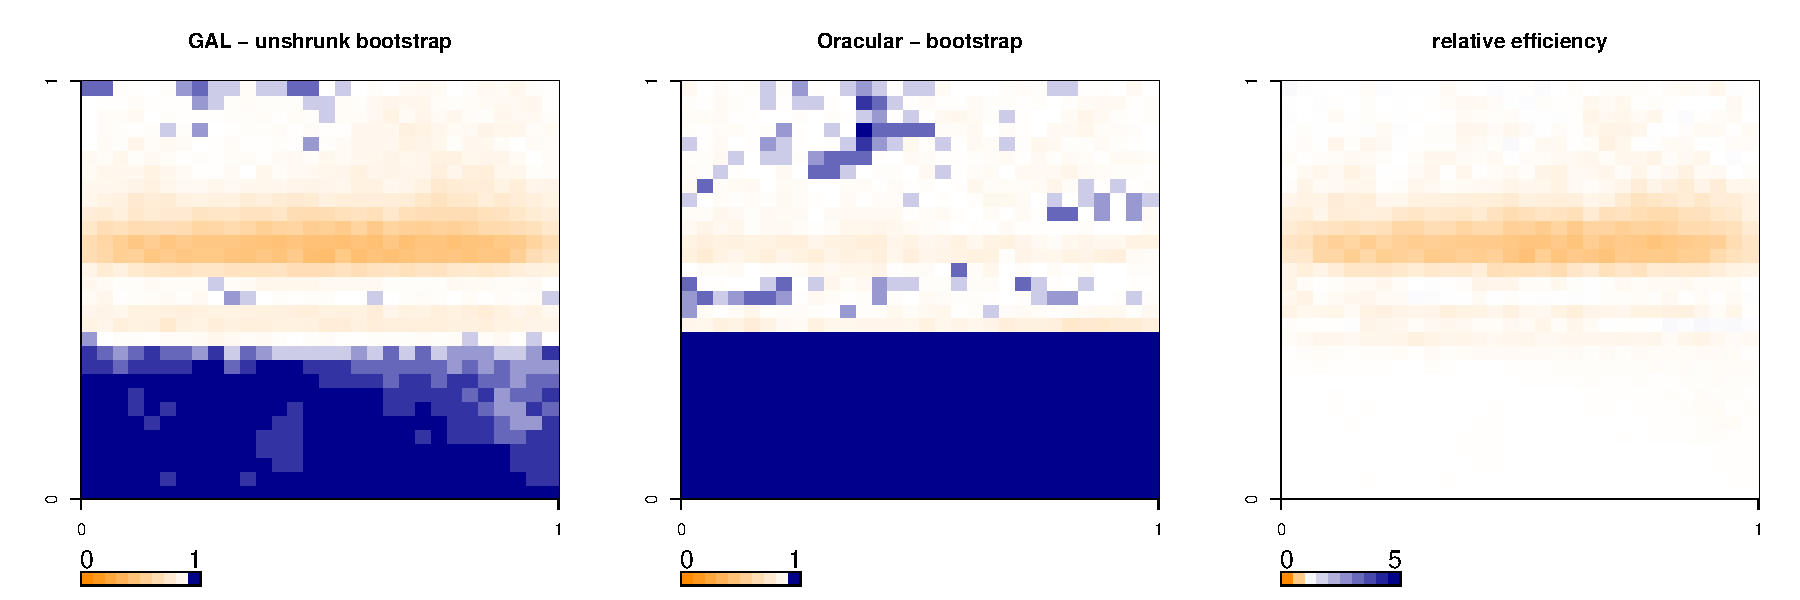
\includegraphics[width=0.99\textwidth]{../../figures/X1-28-5.pdf}
		%\includegraphics[width=\textwidth]{../../figures/simulation/28-2-profile-coverage.pdf}
		\captionof{figure}{Coverage frequency of 95\% CIs: setting 5}
		\label{fig:coveragemap5}
	\end{center}
	
	\begin{center}
		%\centering
		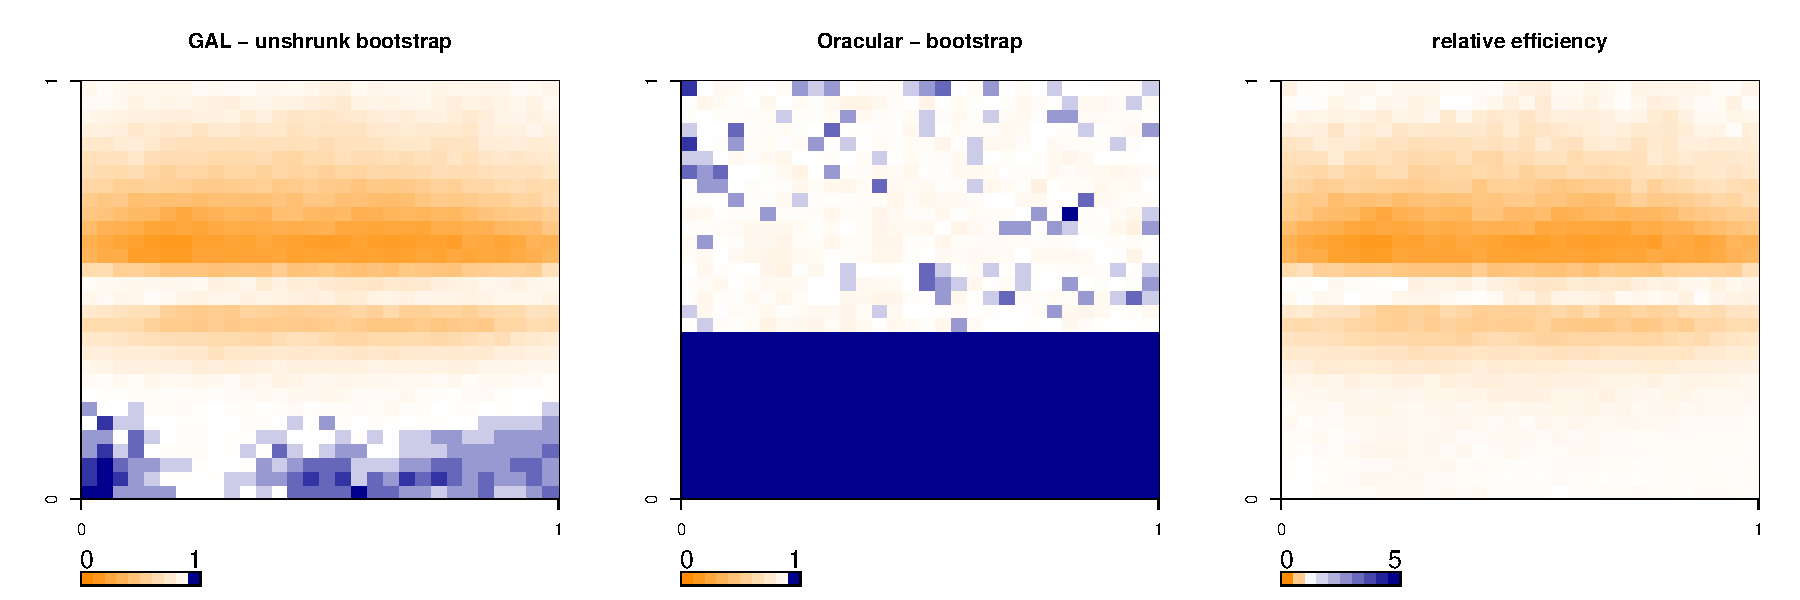
\includegraphics[width=0.99\textwidth]{../../figures/X1-28-6.pdf}
		%\includegraphics[width=\textwidth]{../../figures/simulation/28-3-profile-coverage.pdf}
		\captionof{figure}{Coverage frequency of 95\% CIs: setting 6}
		\label{fig:coveragemap6}
	\end{center}
	
	\begin{center}
		%\centering
		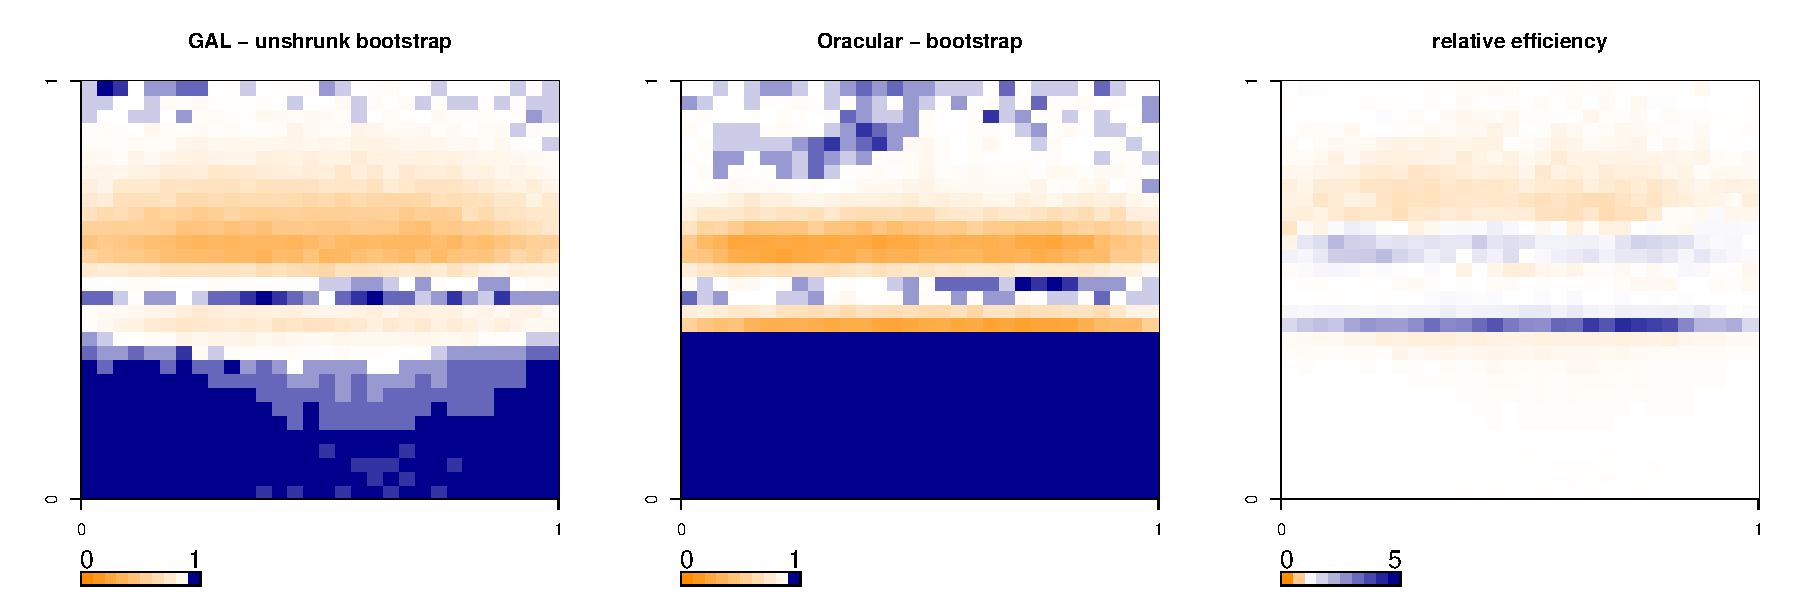
\includegraphics[width=0.99\textwidth]{../../figures/X1-28-7.pdf}
		%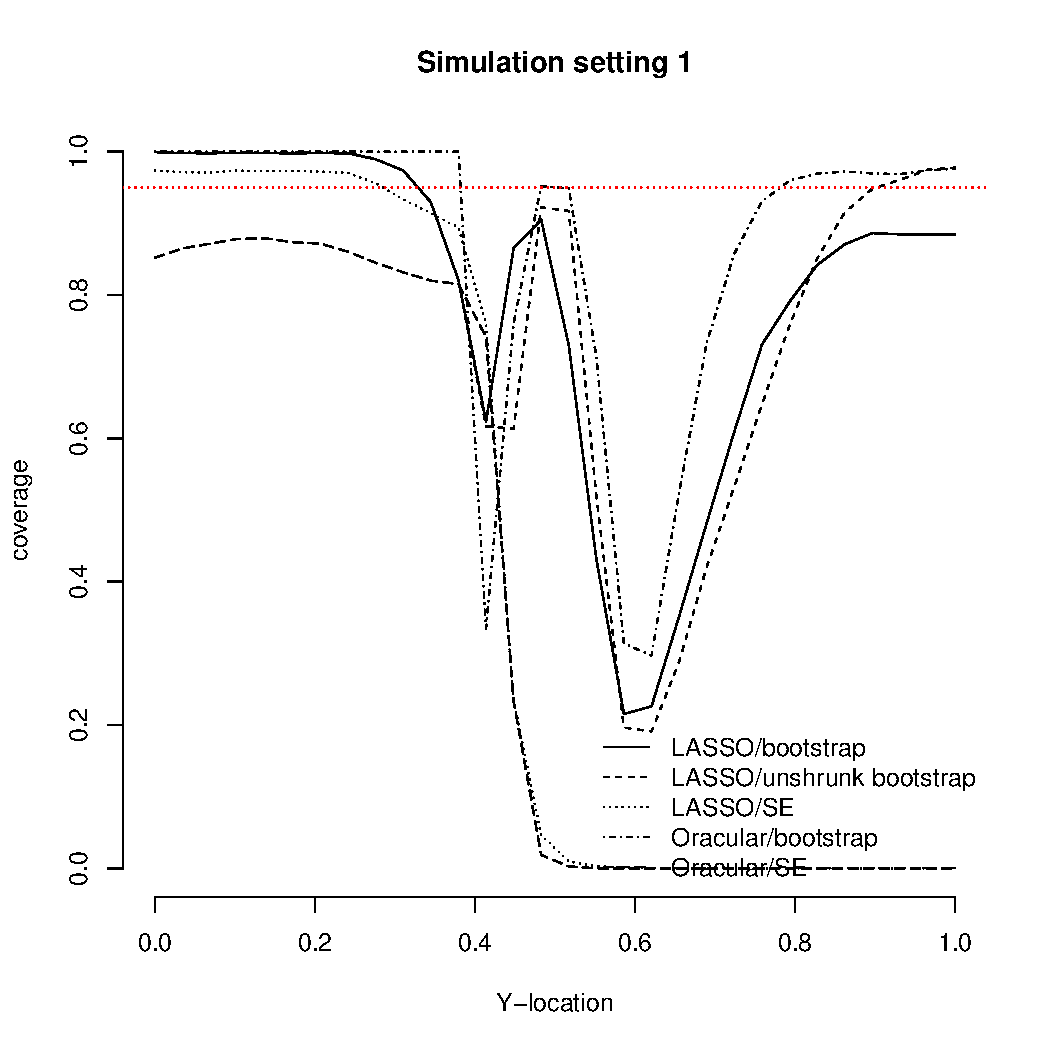
\includegraphics[width=\textwidth]{../../figures/simulation/28-1-profile-coverage.pdf}
		\captionof{figure}{Coverage frequency of 95\% CIs: setting 7}
		\label{fig:coveragemap7}
	\end{center}
		        
	\begin{center}
		%\centering
		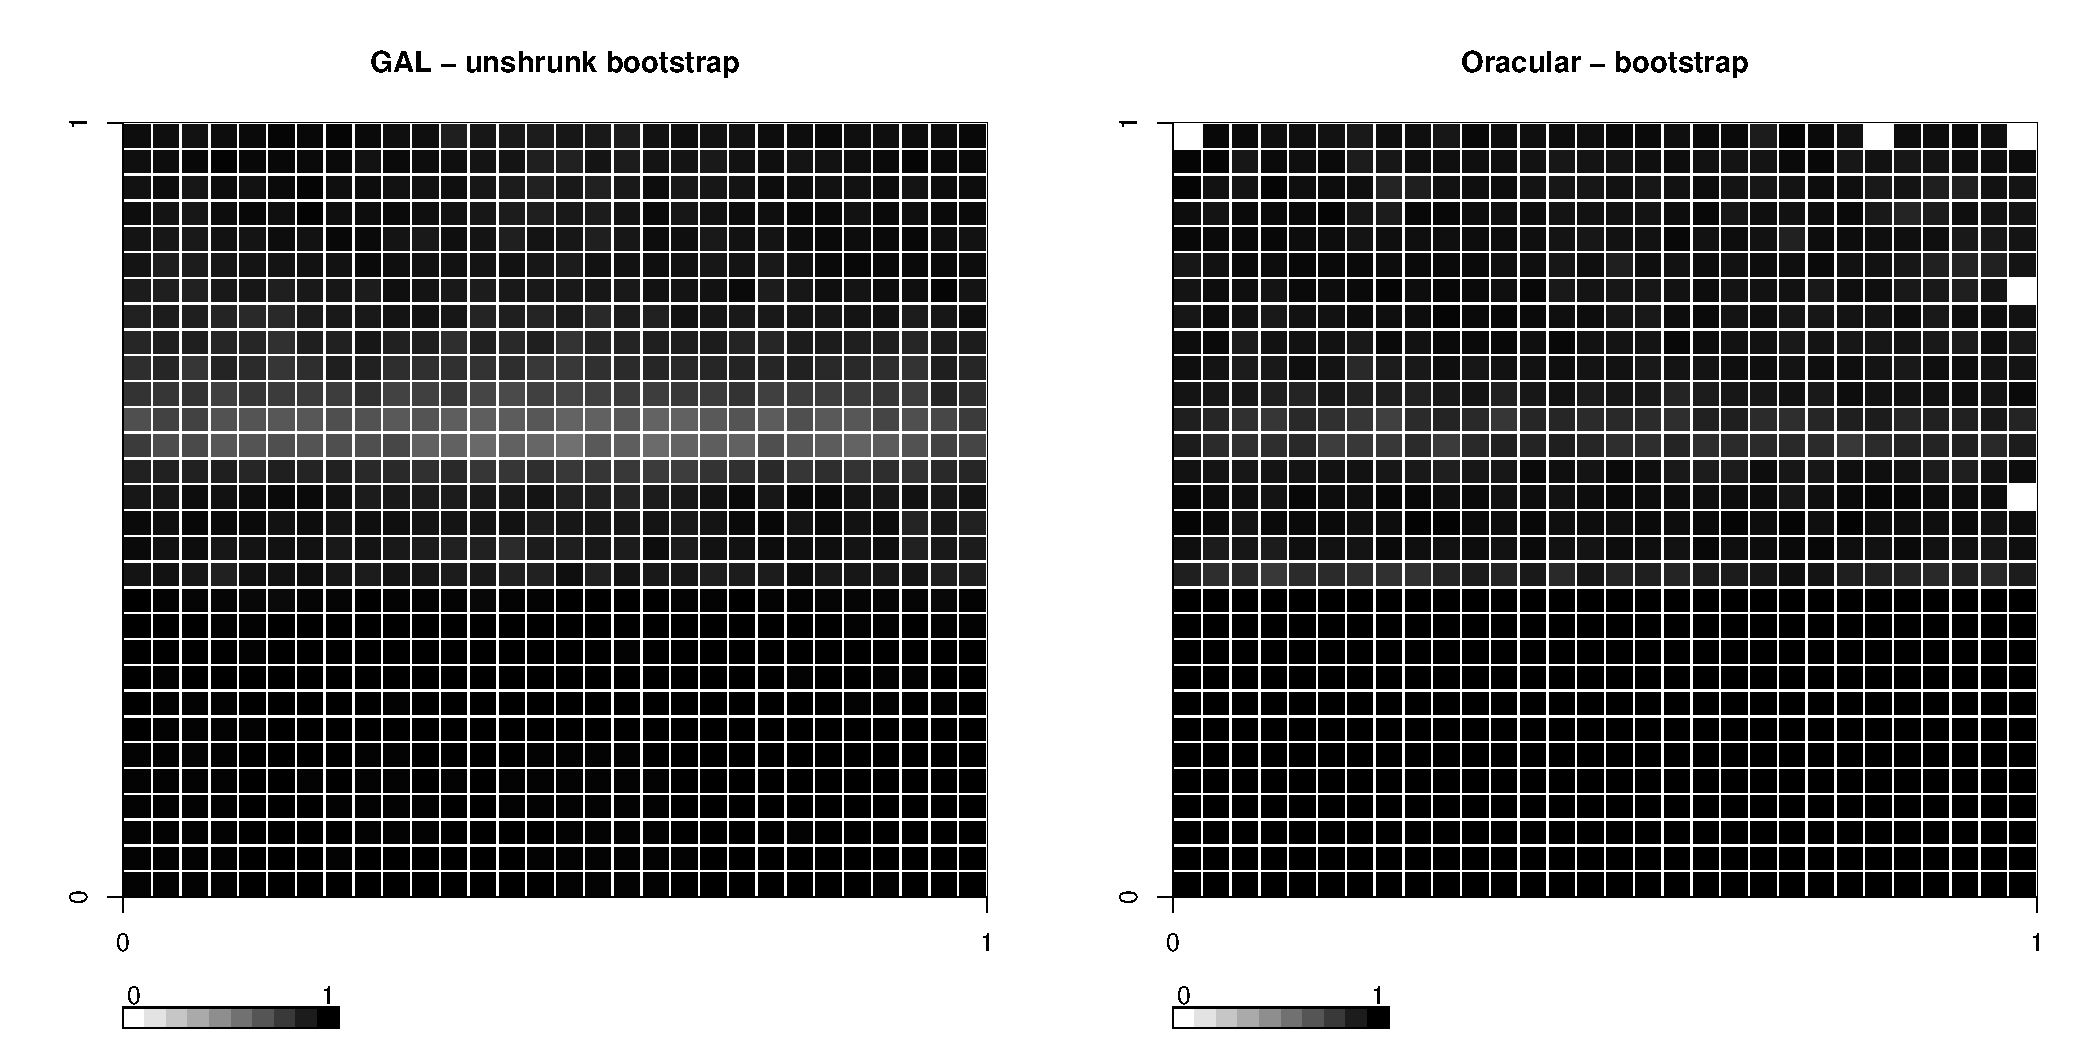
\includegraphics[width=0.99\textwidth]{../../figures/X1-28-8.pdf}
		%\includegraphics[width=\textwidth]{../../figures/simulation/28-2-profile-coverage.pdf}
		\captionof{figure}{Coverage frequency of 95\% CIs: setting 8}
		\label{fig:coveragemap8}
	\end{center}
	
	\begin{center}
		%\centering
		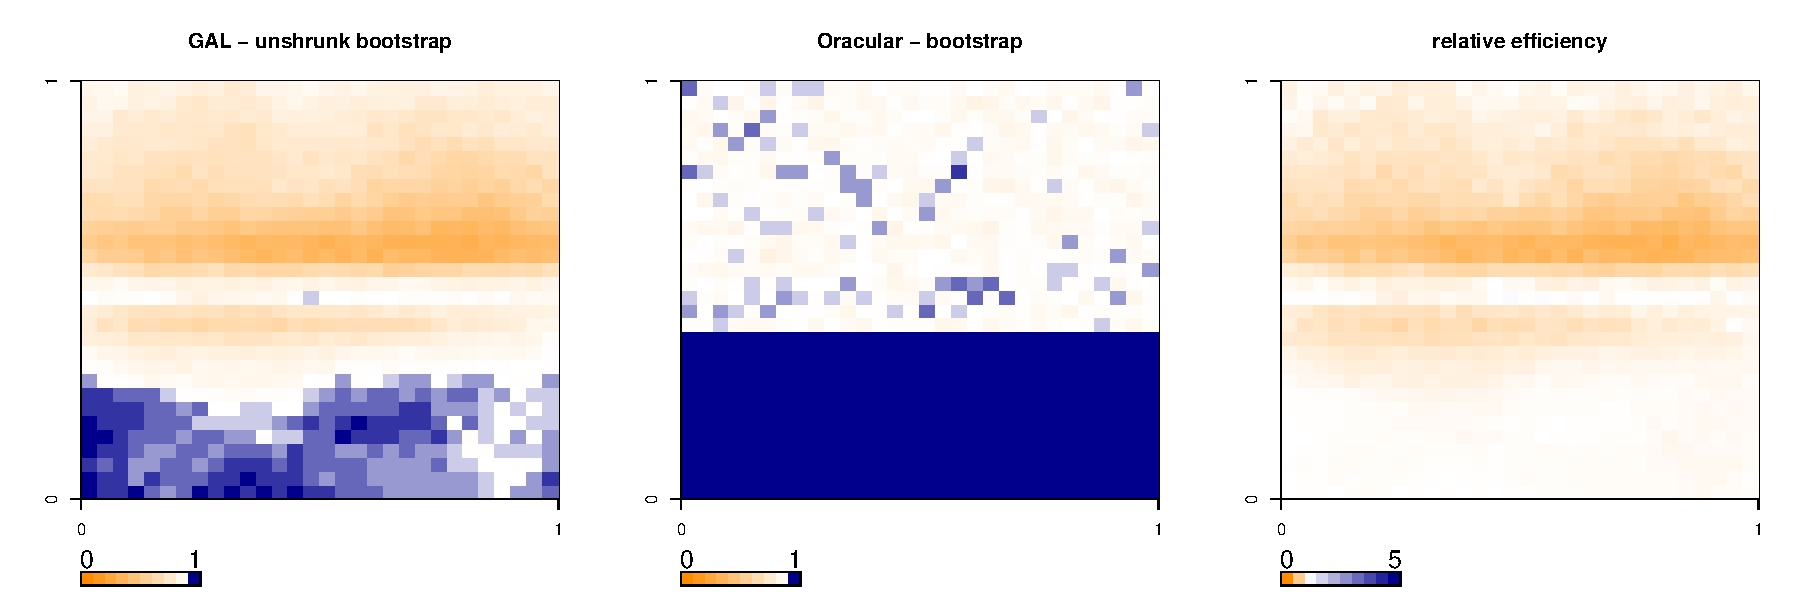
\includegraphics[width=0.99\textwidth]{../../figures/X1-28-9.pdf}
		%\includegraphics[width=\textwidth]{../../figures/simulation/28-3-profile-coverage.pdf}
		\captionof{figure}{Coverage frequency of 95\% CIs: setting 9}
		\label{fig:coveragemap9}
	\end{center}
	
	\begin{center}
		%\centering
		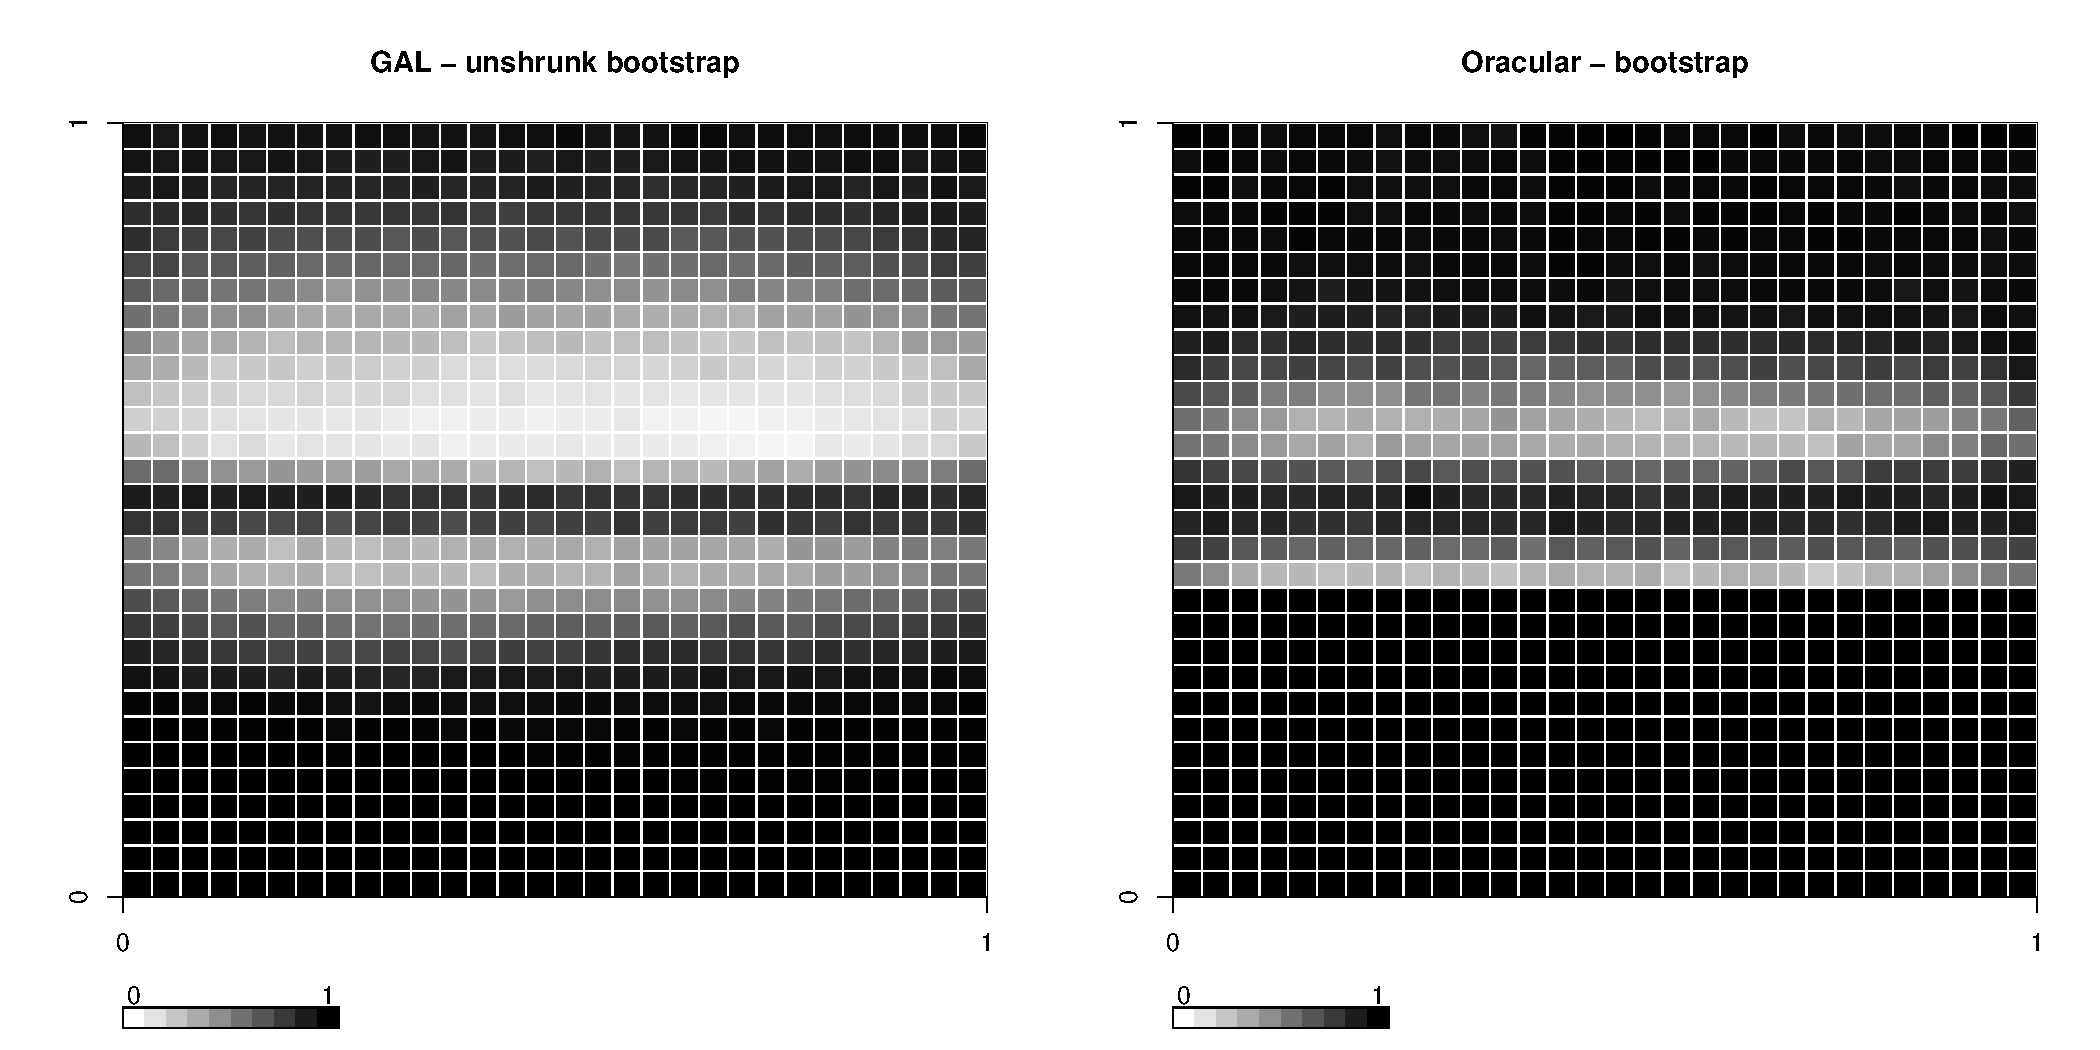
\includegraphics[width=0.99\textwidth]{../../figures/X1-28-10.pdf}
		%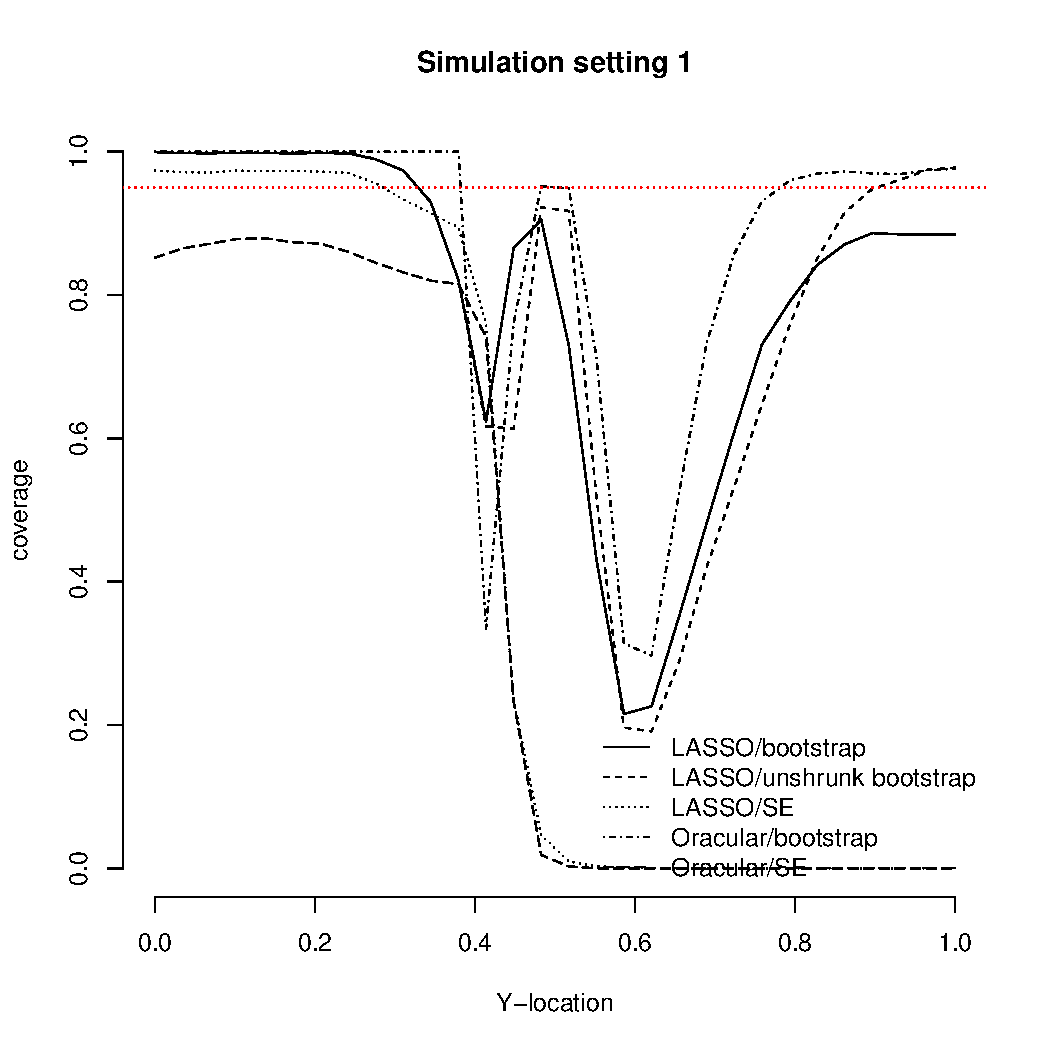
\includegraphics[width=\textwidth]{../../figures/simulation/28-1-profile-coverage.pdf}
		\captionof{figure}{Coverage frequency of 95\% CIs: setting 10}
		\label{fig:coveragemap10}
	\end{center}
        
	\begin{center}
		%\centering
		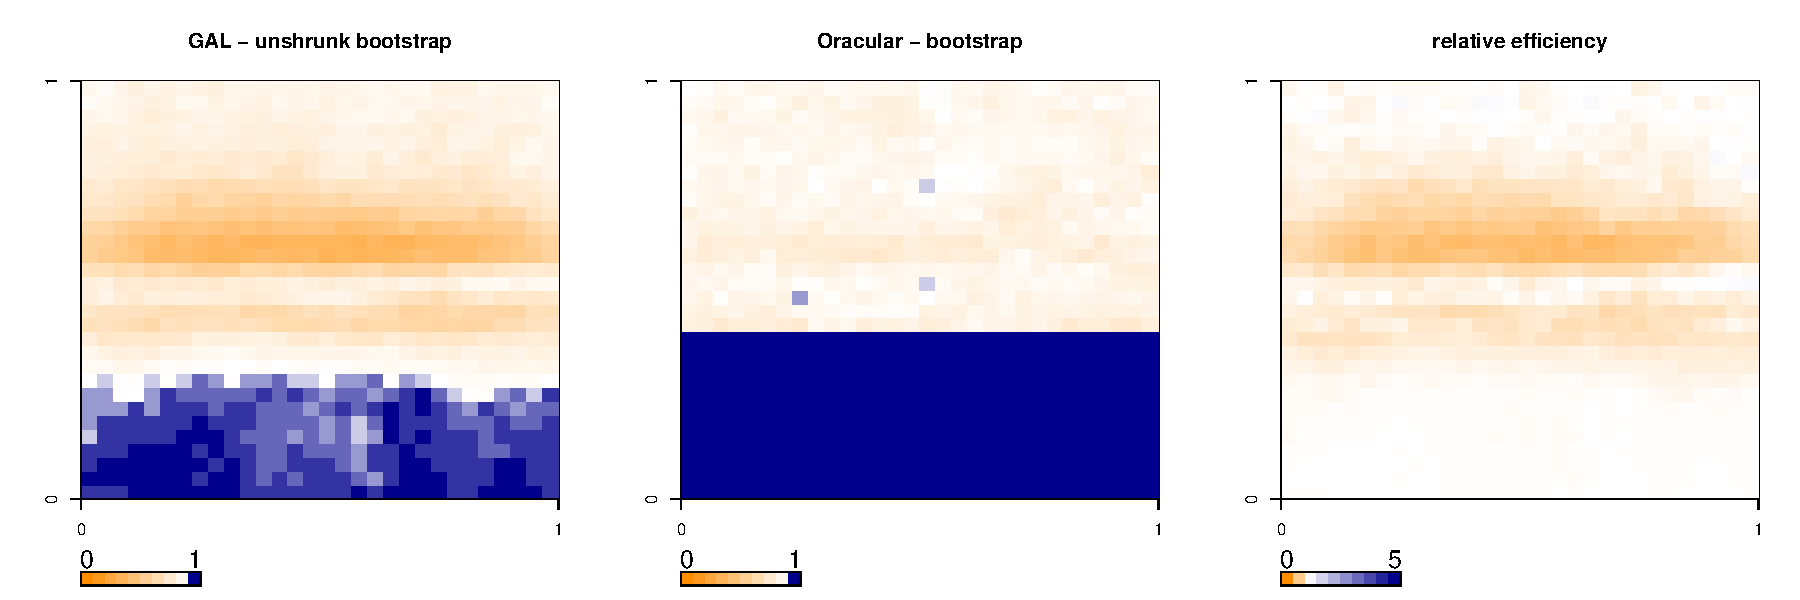
\includegraphics[width=0.99\textwidth]{../../figures/X1-28-11.pdf}
		%\includegraphics[width=\textwidth]{../../figures/simulation/28-2-profile-coverage.pdf}
		\captionof{figure}{Coverage frequency of 95\% CIs: setting 11}
		\label{fig:coveragemap11}
	\end{center}
	
	\begin{center}
		%\centering
		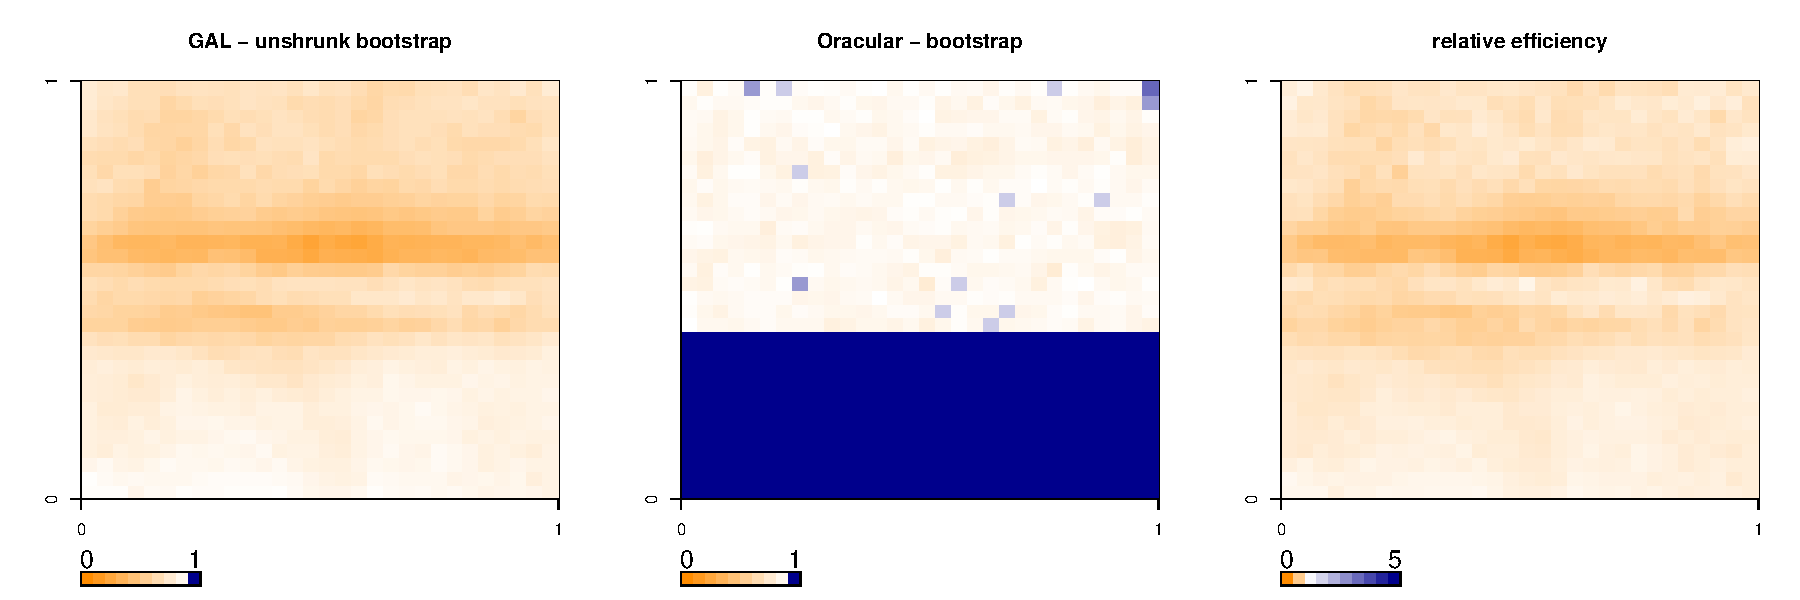
\includegraphics[width=0.99\textwidth]{../../figures/X1-28-12.pdf}
		%\includegraphics[width=\textwidth]{../../figures/simulation/28-3-profile-coverage.pdf}
		\captionof{figure}{Coverage frequency of 95\% CIs: setting 12}
		\label{fig:coveragemap12}
	\end{center}
	
	\begin{center}
		%\centering
		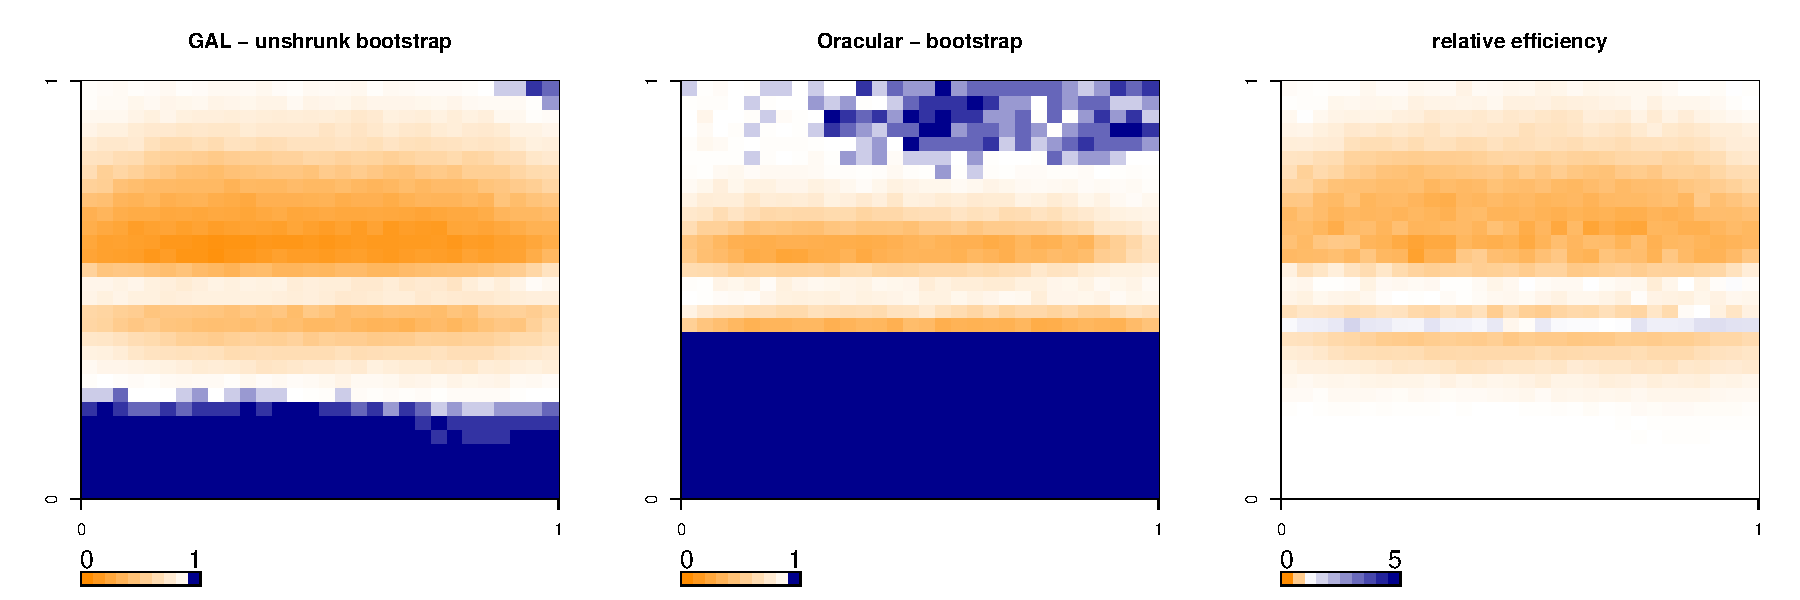
\includegraphics[width=0.99\textwidth]{../../figures/X1-28-13.pdf}
		%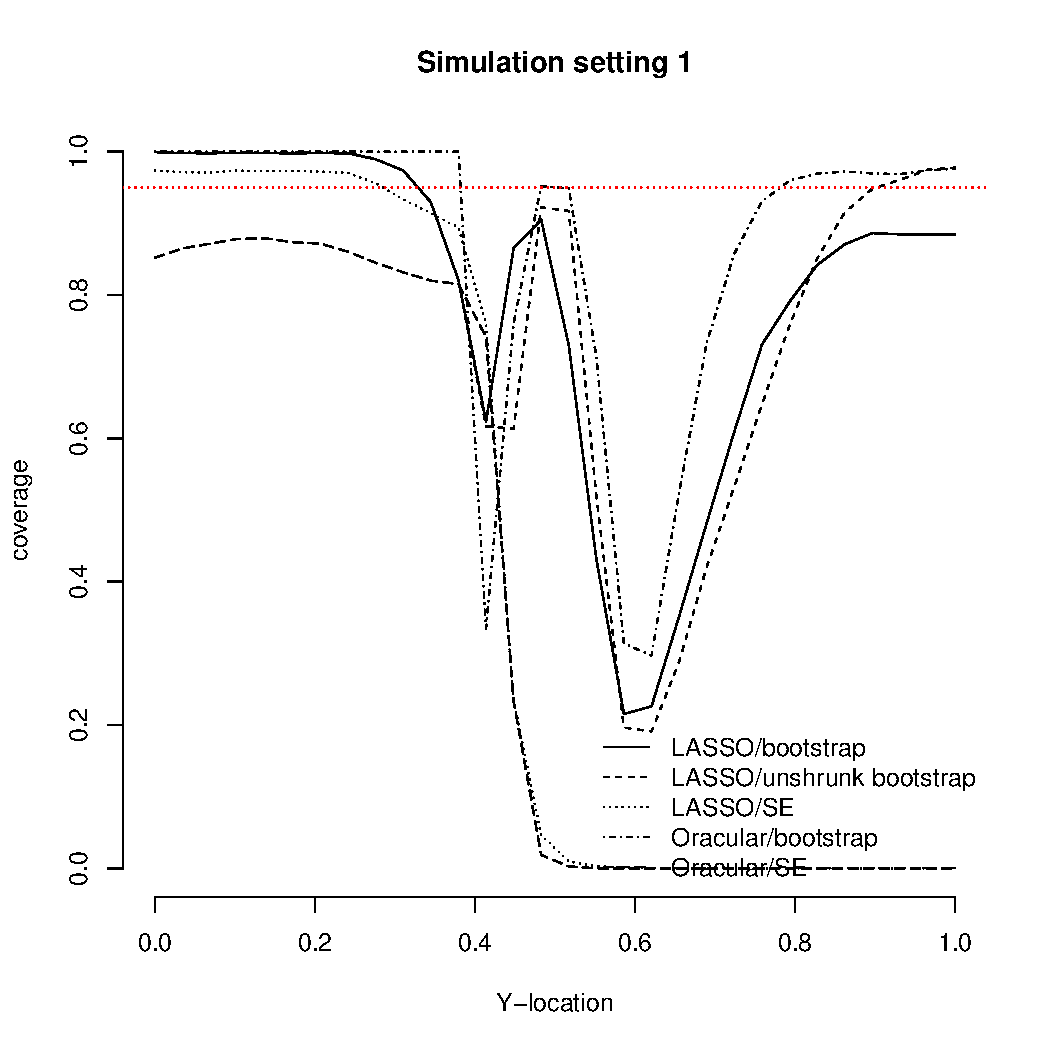
\includegraphics[width=\textwidth]{../../figures/simulation/28-1-profile-coverage.pdf}
		\captionof{figure}{Coverage frequency of 95\% CIs: setting 13}
		\label{fig:coveragemap13}
	\end{center}
        
	\begin{center}
		%\centering
		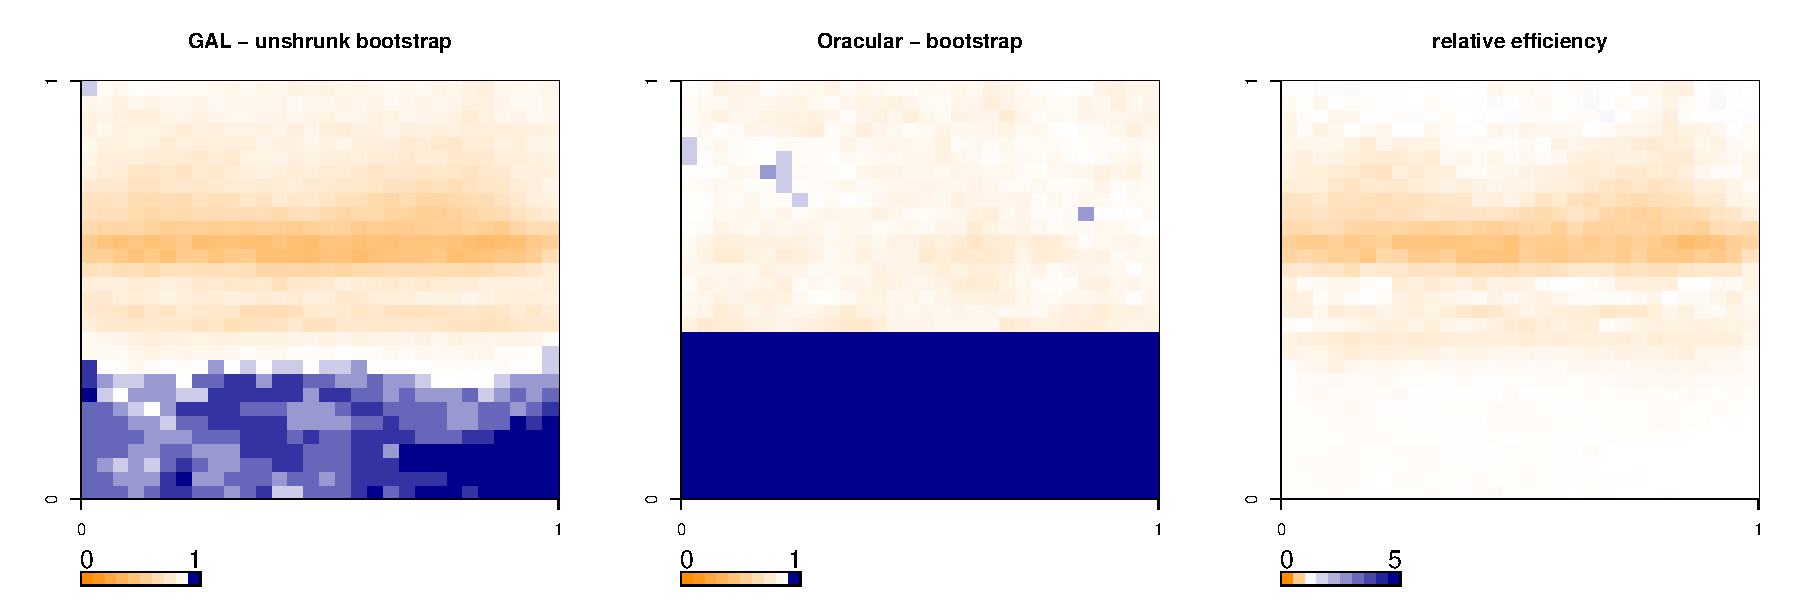
\includegraphics[width=0.99\textwidth]{../../figures/X1-28-14.pdf}
		%\includegraphics[width=\textwidth]{../../figures/simulation/28-2-profile-coverage.pdf}
		\captionof{figure}{Coverage frequency of 95\% CIs: setting 14}
		\label{fig:coveragemap14}
	\end{center}
	
	\begin{center}
		%\centering
		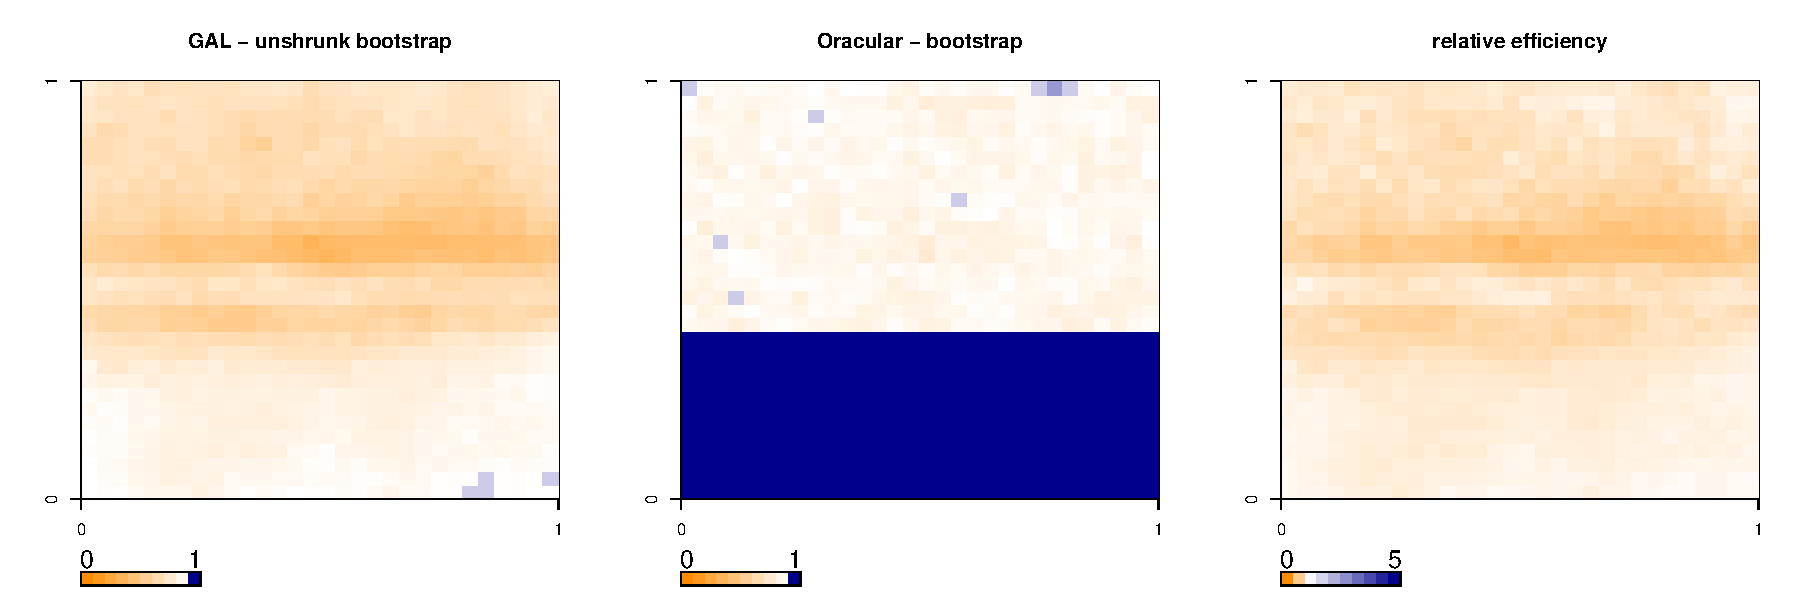
\includegraphics[width=0.99\textwidth]{../../figures/X1-28-15.pdf}
		%\includegraphics[width=\textwidth]{../../figures/simulation/28-3-profile-coverage.pdf}
		\captionof{figure}{Coverage frequency of 95\% CIs: setting 15}
		\label{fig:coveragemap15}
	\end{center}
	
	\begin{center}
		%\centering
		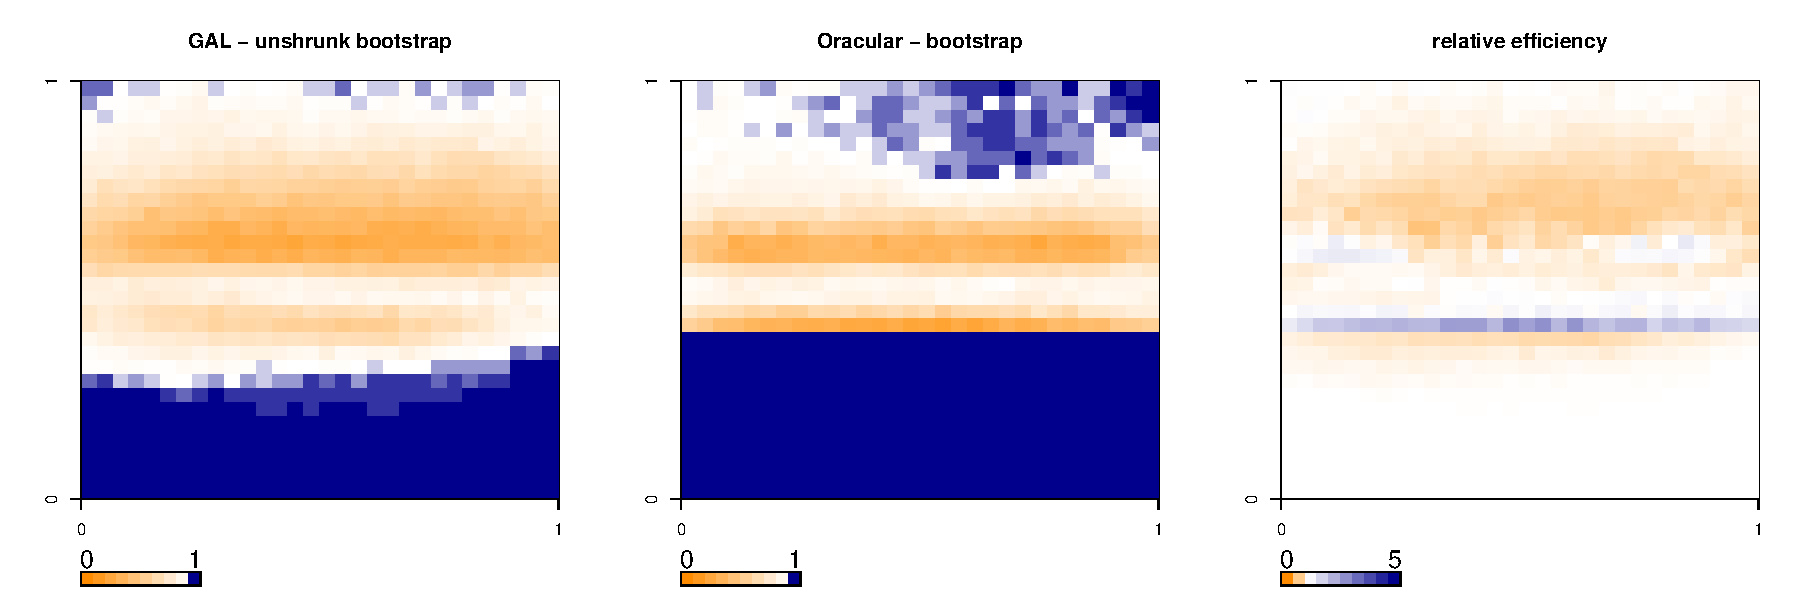
\includegraphics[width=0.99\textwidth]{../../figures/X1-28-16.pdf}
		%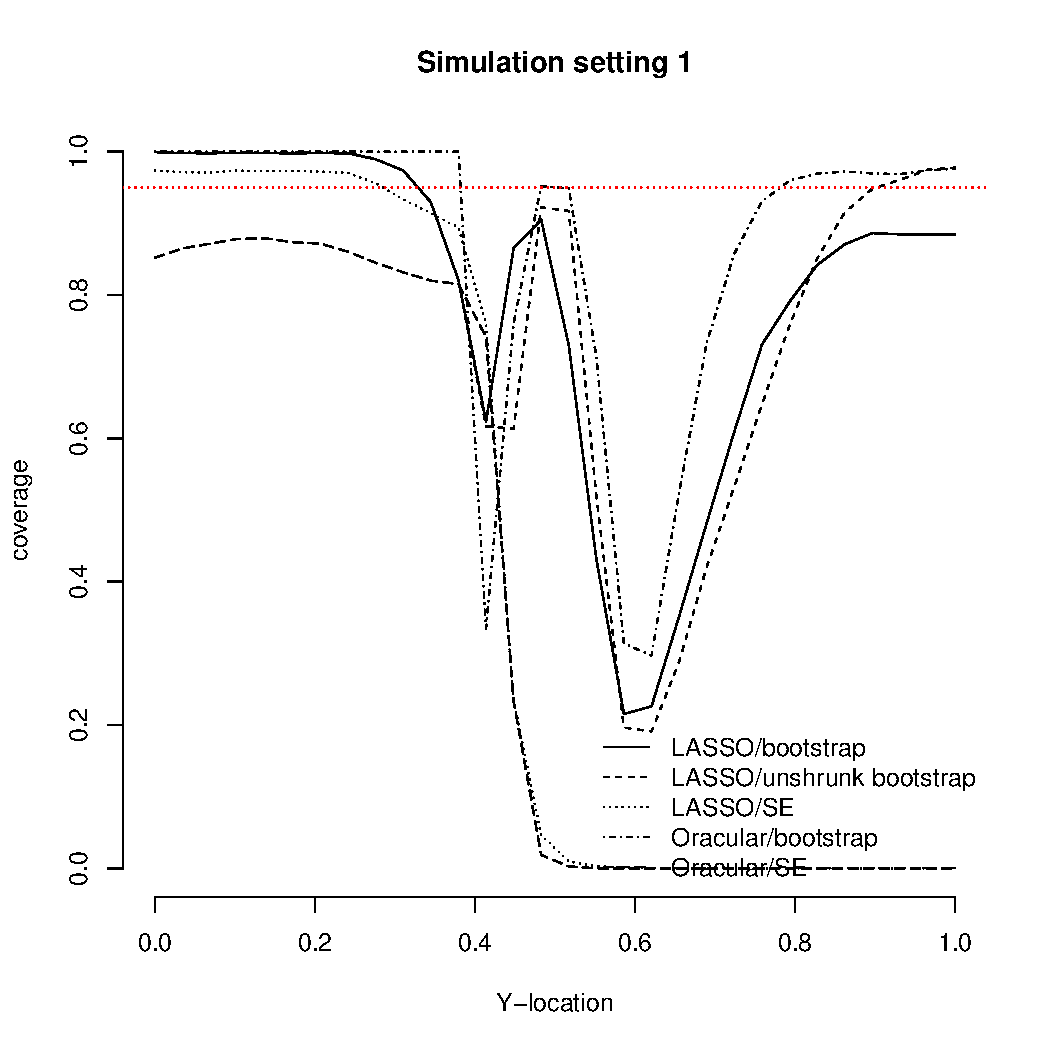
\includegraphics[width=\textwidth]{../../figures/simulation/28-1-profile-coverage.pdf}
		\captionof{figure}{Coverage frequency of 95\% CIs: setting 16}
		\label{fig:coveragemap16}
	\end{center}
        
	\begin{center}
		%\centering
		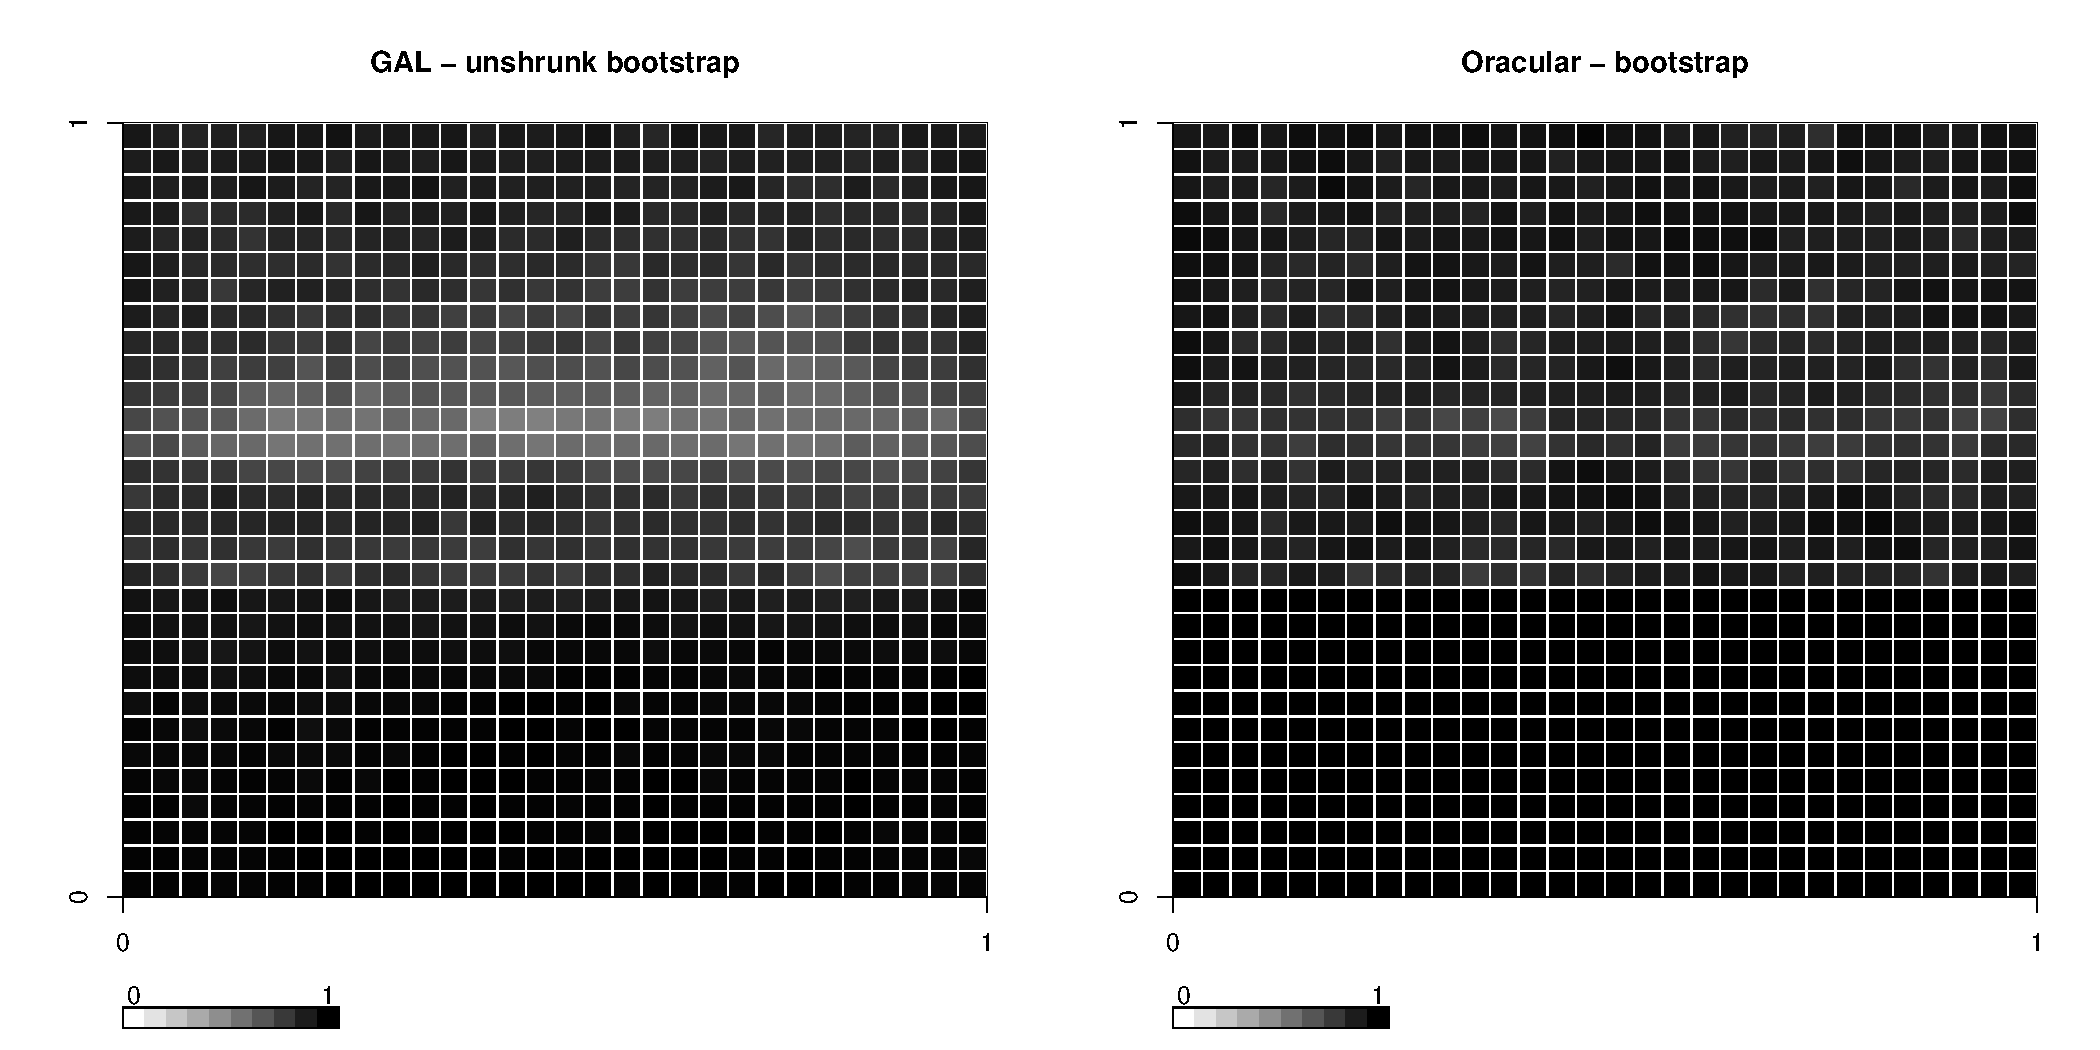
\includegraphics[width=0.99\textwidth]{../../figures/X1-28-17.pdf}
		%\includegraphics[width=\textwidth]{../../figures/simulation/28-2-profile-coverage.pdf}
		\captionof{figure}{Coverage frequency of 95\% CIs: setting 17}
		\label{fig:coveragemap17}
	\end{center}
	
	\begin{center}
		%\centering
		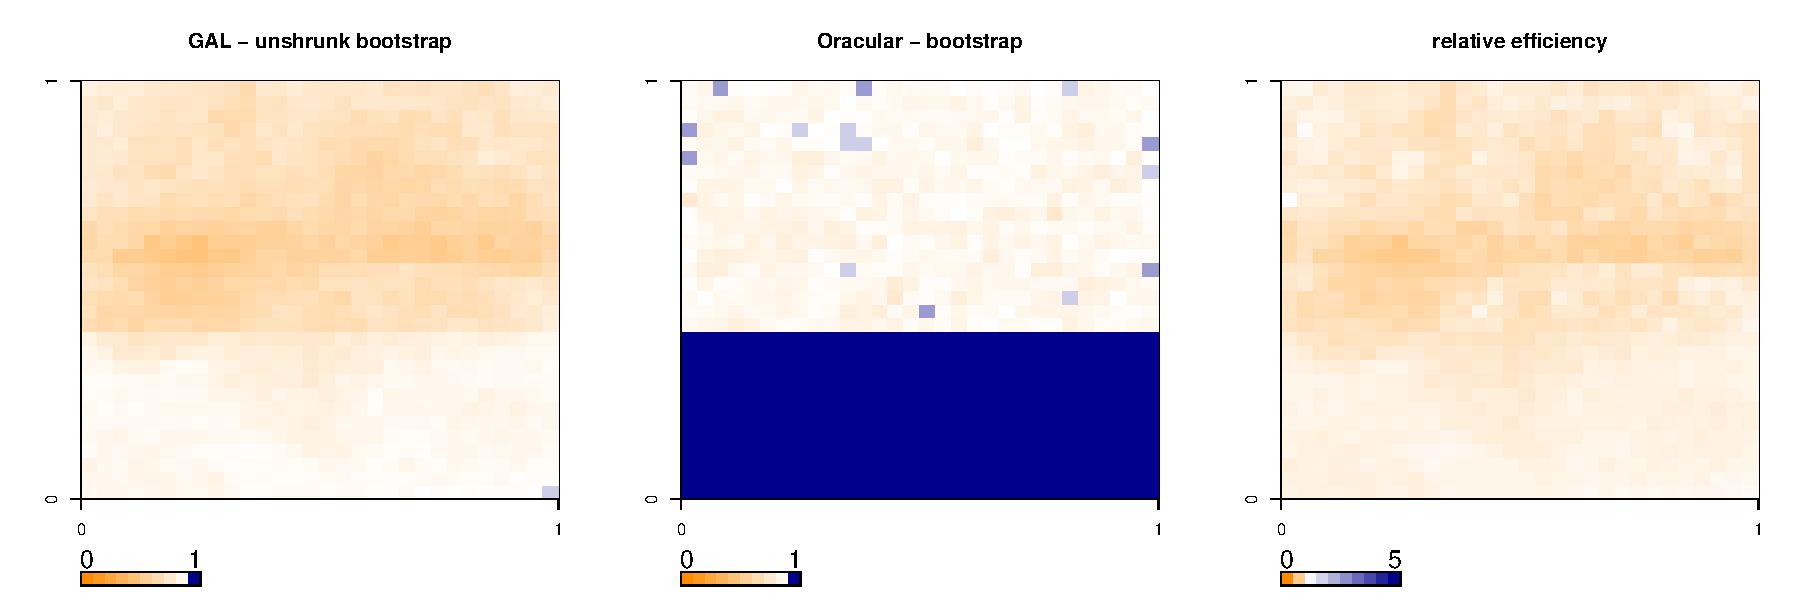
\includegraphics[width=0.99\textwidth]{../../figures/X1-28-18.pdf}
		%\includegraphics[width=\textwidth]{../../figures/simulation/28-3-profile-coverage.pdf}
		\captionof{figure}{Coverage frequency of 95\% CIs: setting 18}
		\label{fig:coveragemap18}
	\end{center}
	
	%\begin{comment}
	%\end{comment}

			
\section{Data analysis}
	\subsection{Census poverty data}
	We present the following analysis to demonstrate one possible application of the geographically-weighted lasso in a linear regression context. We use county-level data from the US Census Bureau to select the social and demographic variables that are important predictors of the county-level poverty rate in the upper midwest, and to estimate the coefficients associated with these predictors. Data are from six censuses - the decennial censuses from 1960 to 2000, and from the American Community Survey in 2006. Selection and estimation are done for each census individually (no attempt is made here to borrow strength across years). The outcome of interest (poverty rate) is a proportion and so takes values on $[0,1]$, but to demonstrate the GAL in a linear regression context, we model the logit-transformed poverty rate. Our data set covers all counties in the states of Minnesota, Iowa, Wisconsin, Illinois, Indiana, and Michigan. The potential predictors are described in Table \ref{table:census-vars}.\\
	
	\begin{table}
		\begin{center}
		\begin{tabular}{ll}
			Variable name & Description \\
			\hline
			\verb!pag! & Proportion working in agriculture\\
			\verb!pex! &  Proportion working in extraction (mining)\\
			\verb!pman! & Proportion working in manufacturing \\
			\verb!pserve! & Proportion working in services \\
			\verb!pfire! & Proportion working in finance, insurance, and real estate \\
			\verb!potprof! & Proportion working in other professions \\
			\verb!pwh! & Proportion who are white \\
			\verb!pblk! & Proportion who are black \\
			\verb!phisp! & Proportion who are hispanic \\
			\verb!metro! & Is the county in a metropolitan area?\\
		\end{tabular}
		\caption{Description of the variables used in the census-data example\label{table:census-vars}}
		\end{center}		
	\end{table}
	
	\subsection{Figures}
	The coefficient estimates are plotted on maps of the upper midwest in Figures \ref{fig:census-coefs-1960} - \ref{fig:census-coefs-2006}. It is immediately apparent that the estimated coefficient surfaces are non-constant for most variables.\\
		
	\begin{figure}
		\begin{center}
			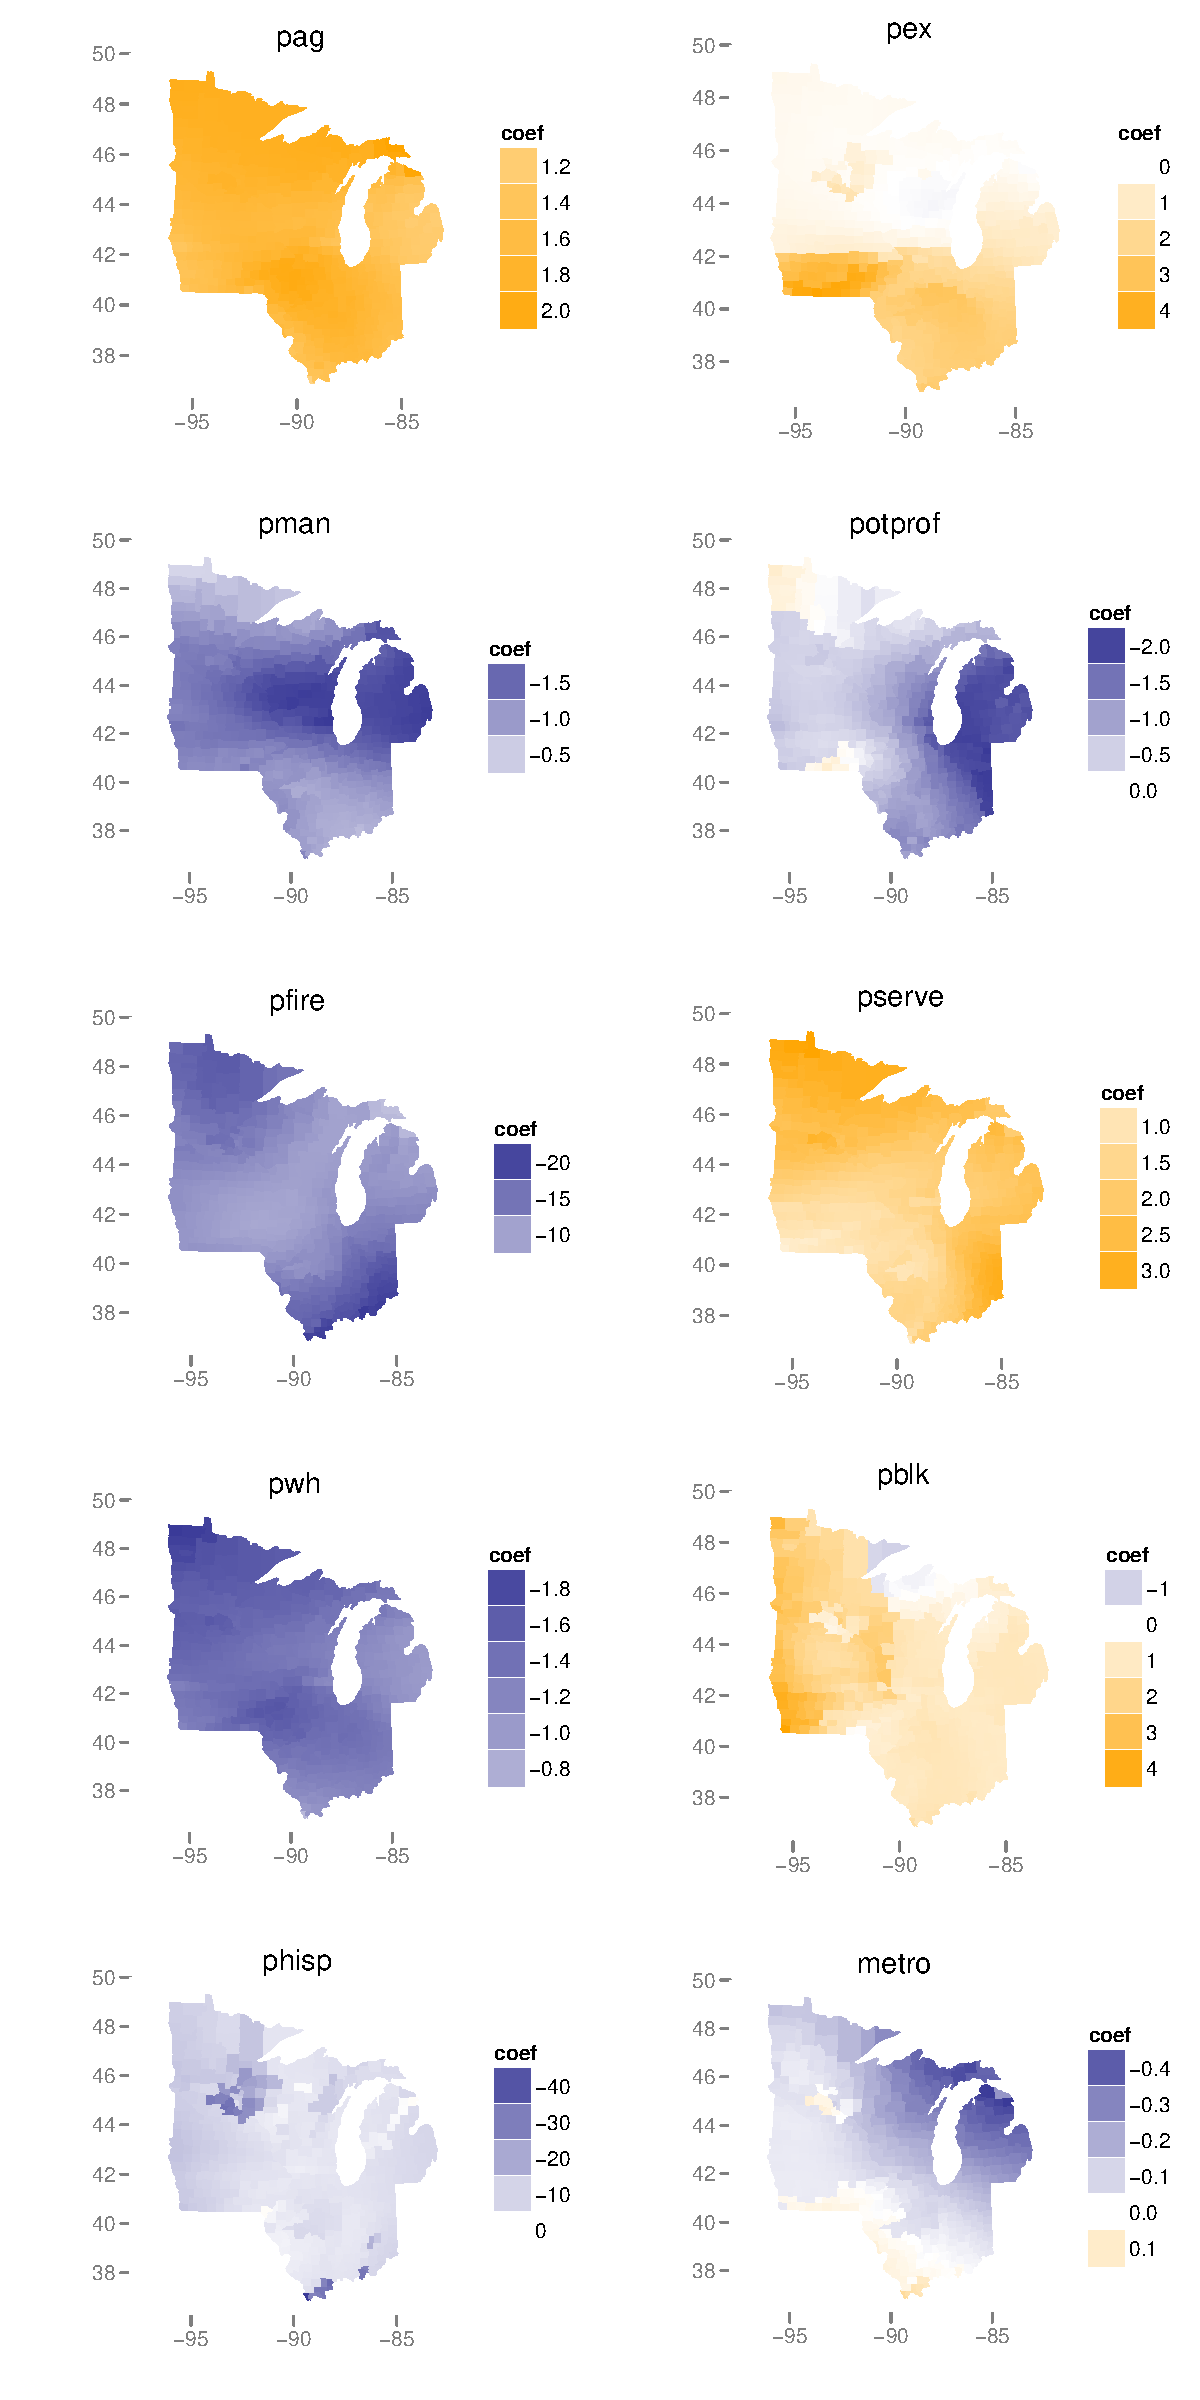
\includegraphics[height=8in]{../../figures/poverty/1960.linear.coefficients.pdf}
			\caption{Estimated coefficient surfaces for the 1960 census.\label{fig:census-coefs-1960}}
		\end{center}		
	\end{figure}

	\begin{figure}
		\begin{center}
			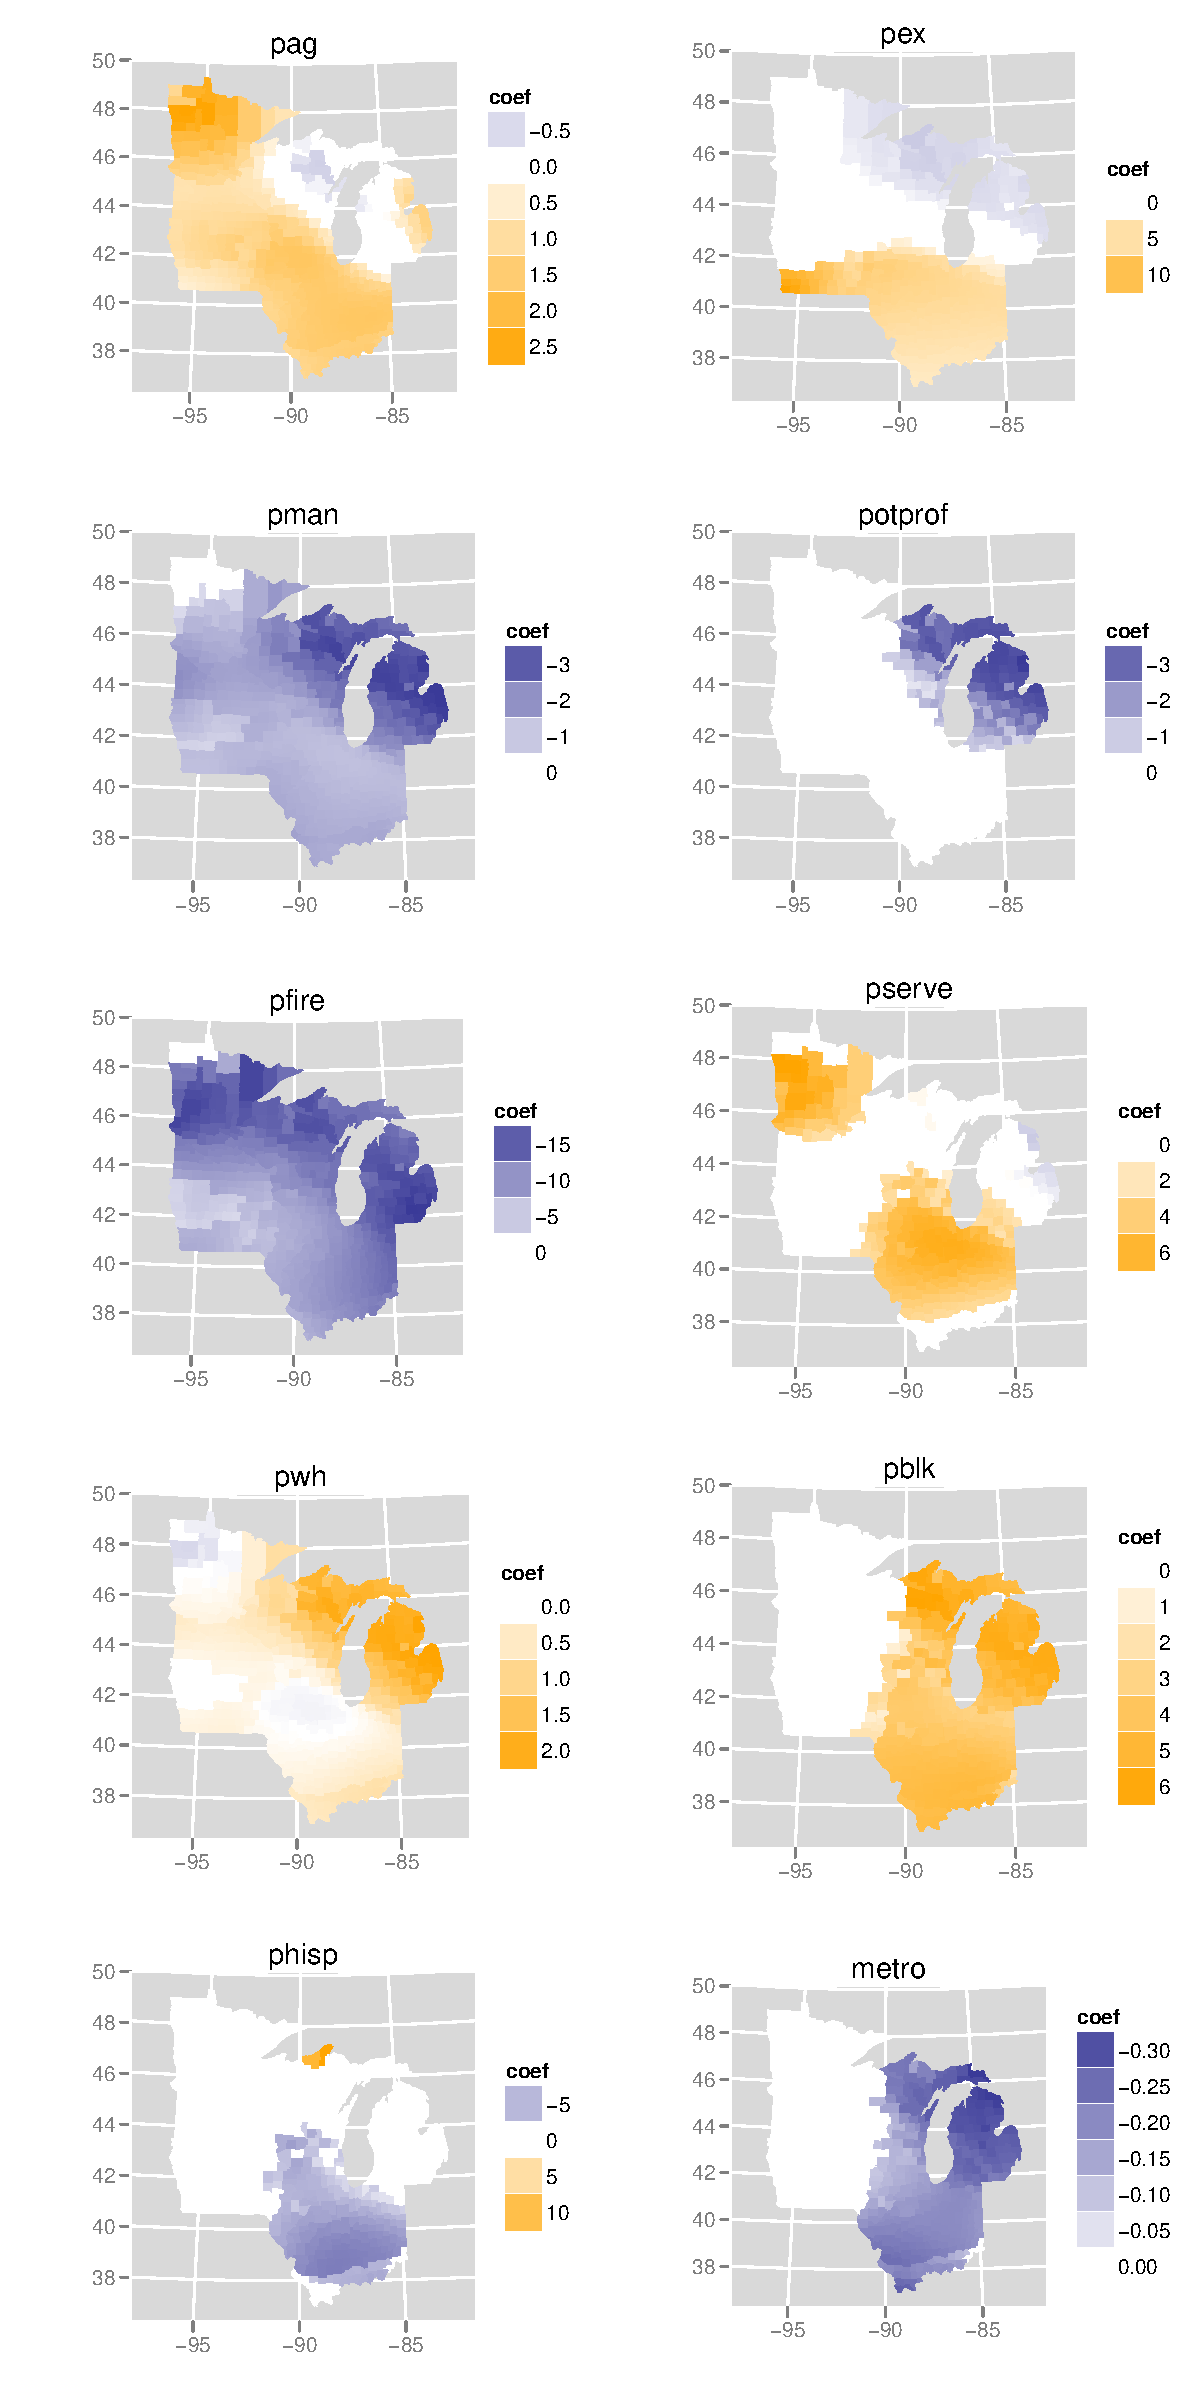
\includegraphics[height=8in]{../../figures/poverty/1970.linear.coefficients.pdf}
			\caption{Estimated coefficient surfaces for the 1970 census.\label{fig:census-coefs-1970}}
		\end{center}
	\end{figure}
	
	\begin{figure}
		\begin{center}
			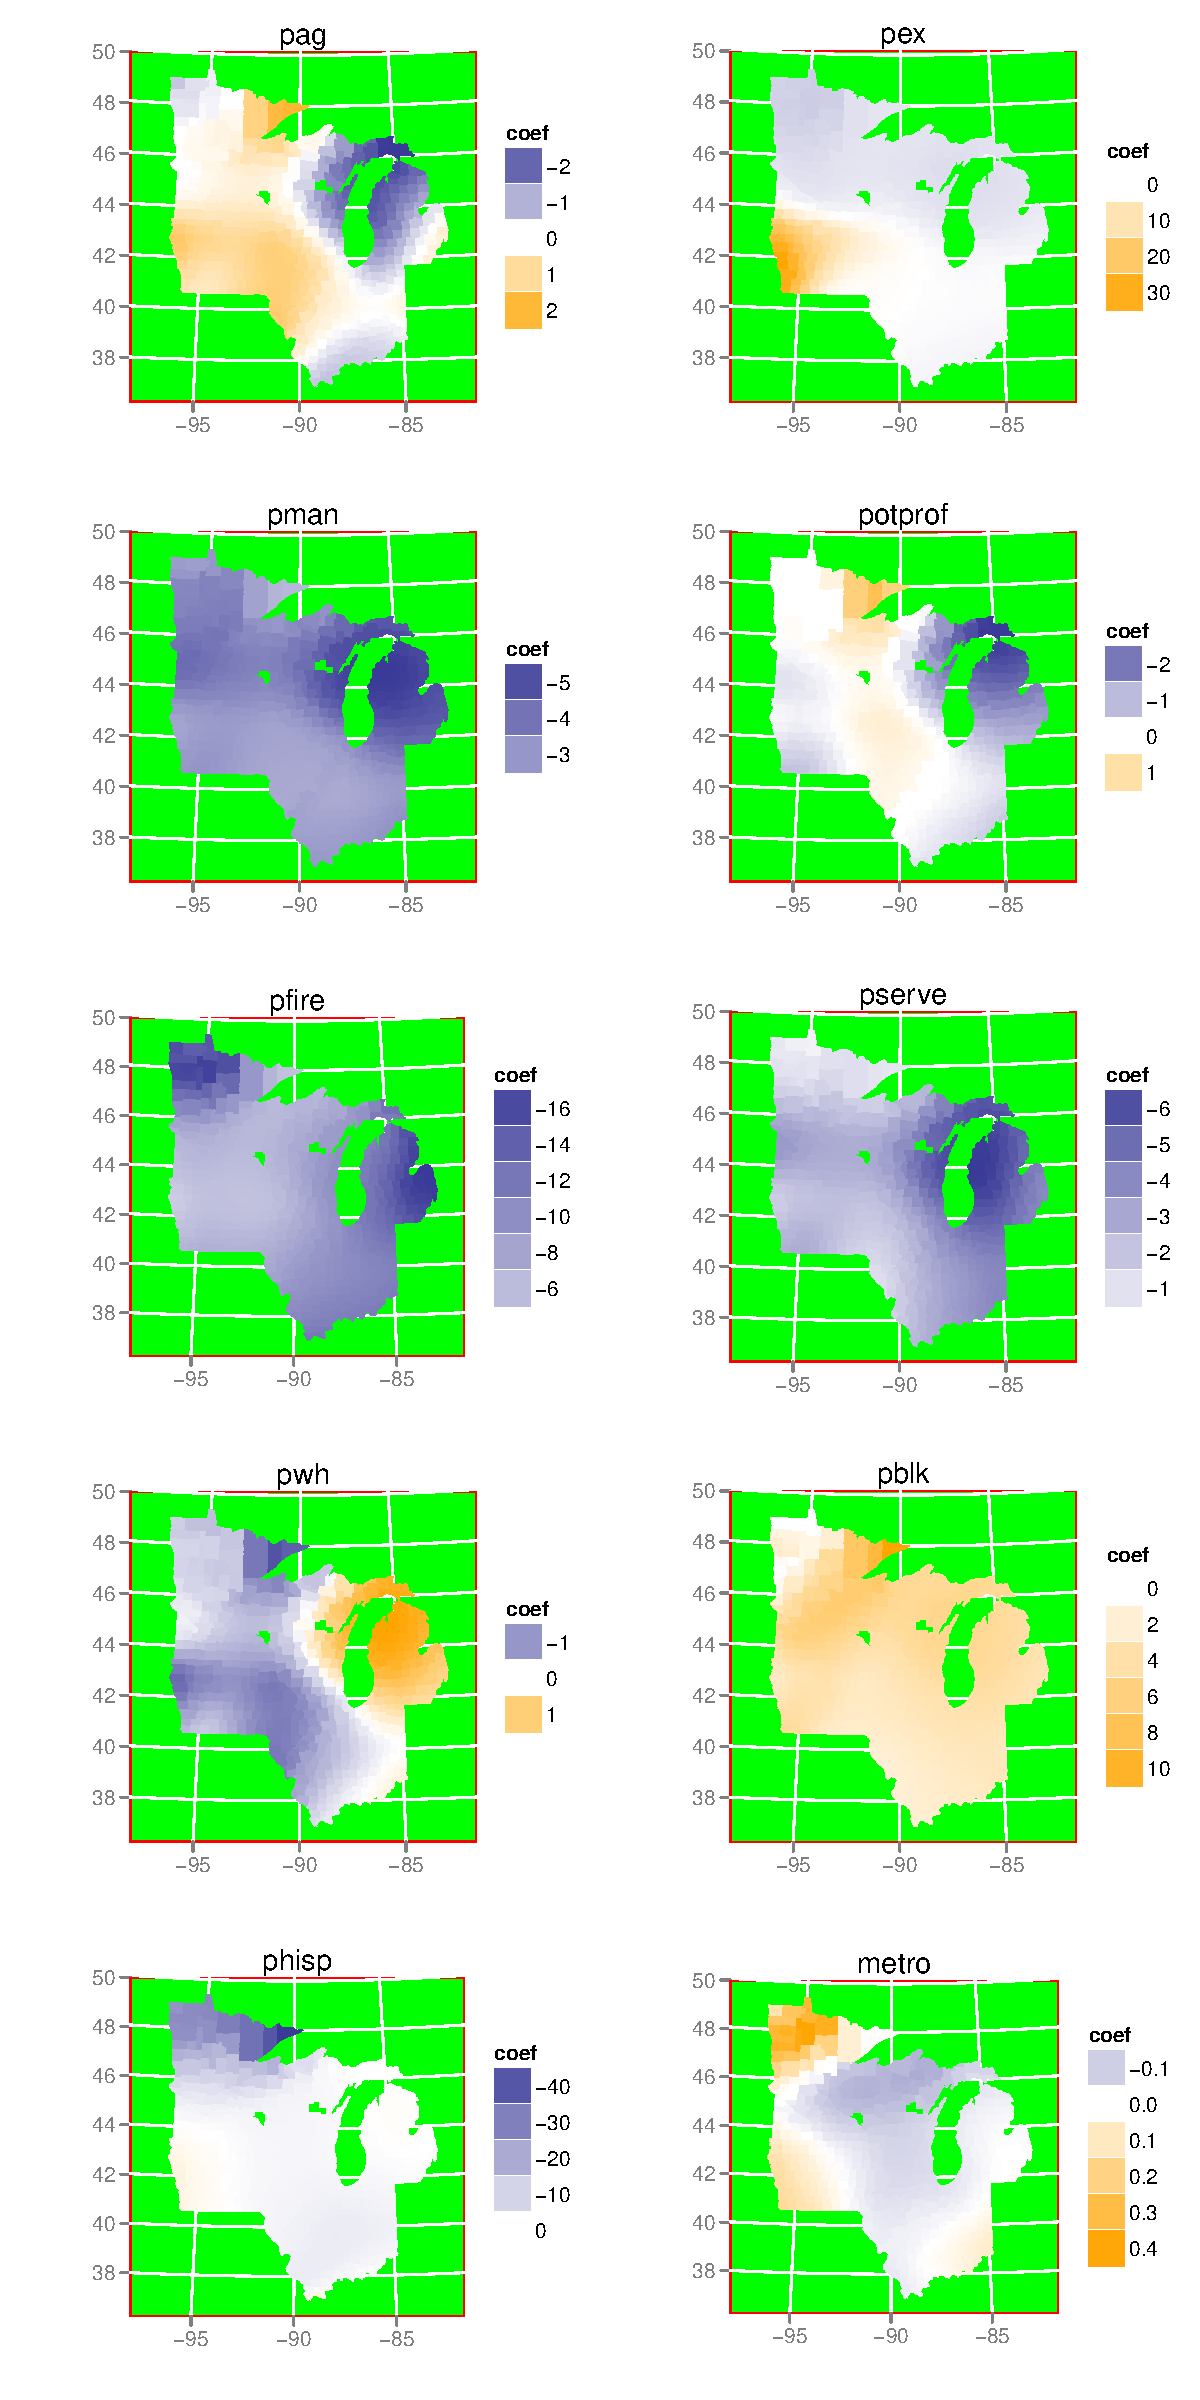
\includegraphics[height=8in]{../../figures/poverty/1980.linear.coefficients.pdf}
			\caption{Estimated coefficient surfaces for the 1980 census.\label{fig:census-coefs-1980}}
		\end{center}
	\end{figure}
	
	\begin{figure}
		\begin{center}
			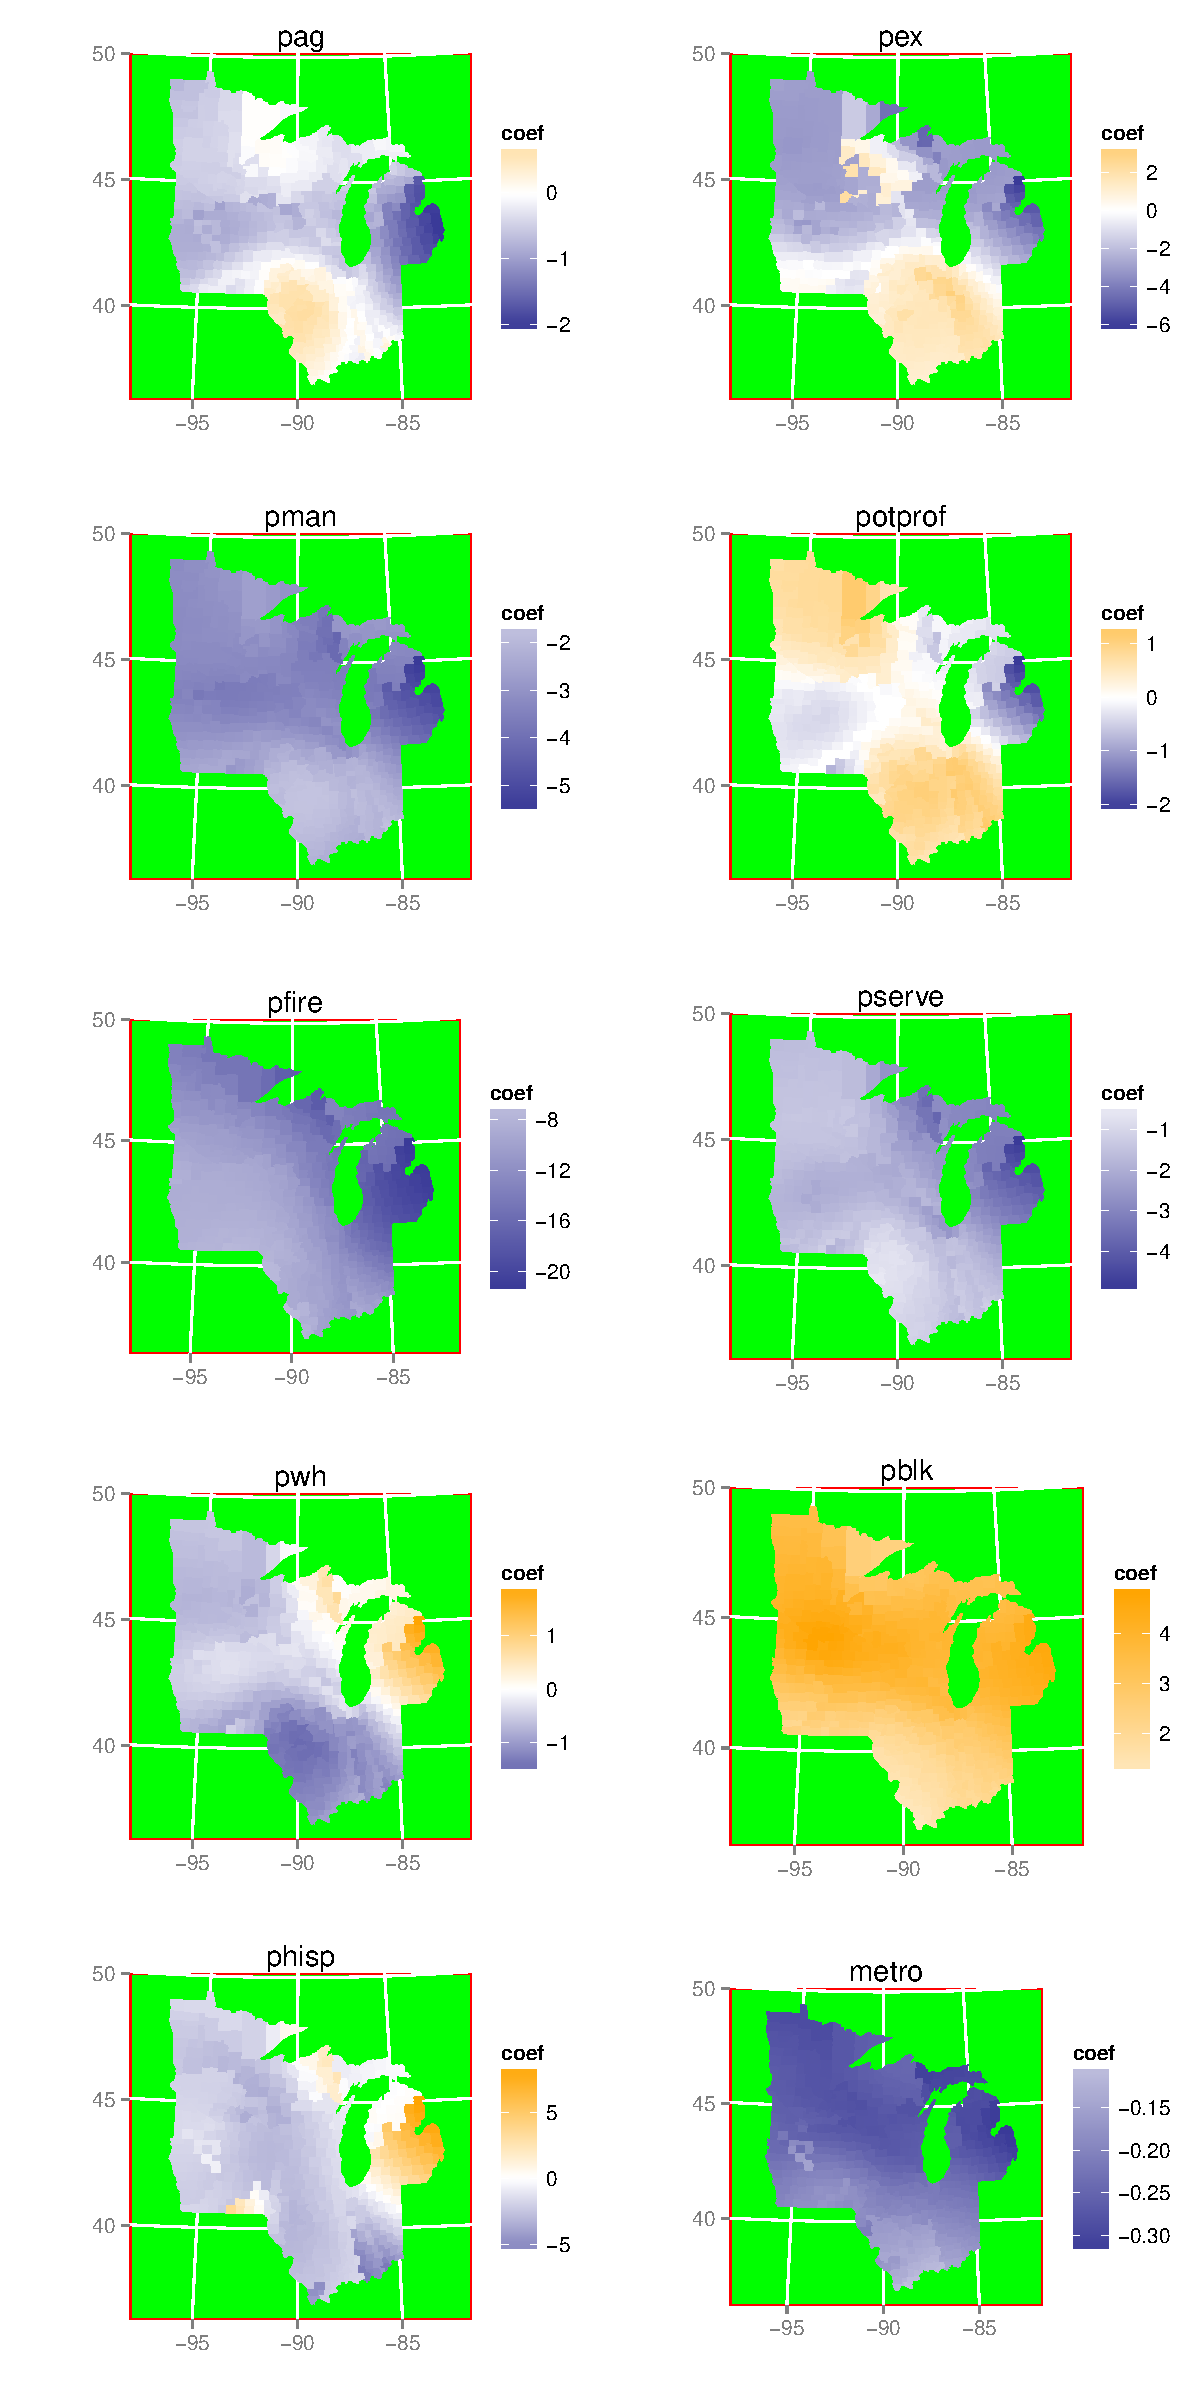
\includegraphics[height=8in]{../../figures/poverty/1990.linear.coefficients.pdf}
			\caption{Estimated coefficient surfaces for the 1990 census.\label{fig:census-coefs-1990}}
		\end{center}
	\end{figure}
	
	\begin{figure}
		\begin{center}
			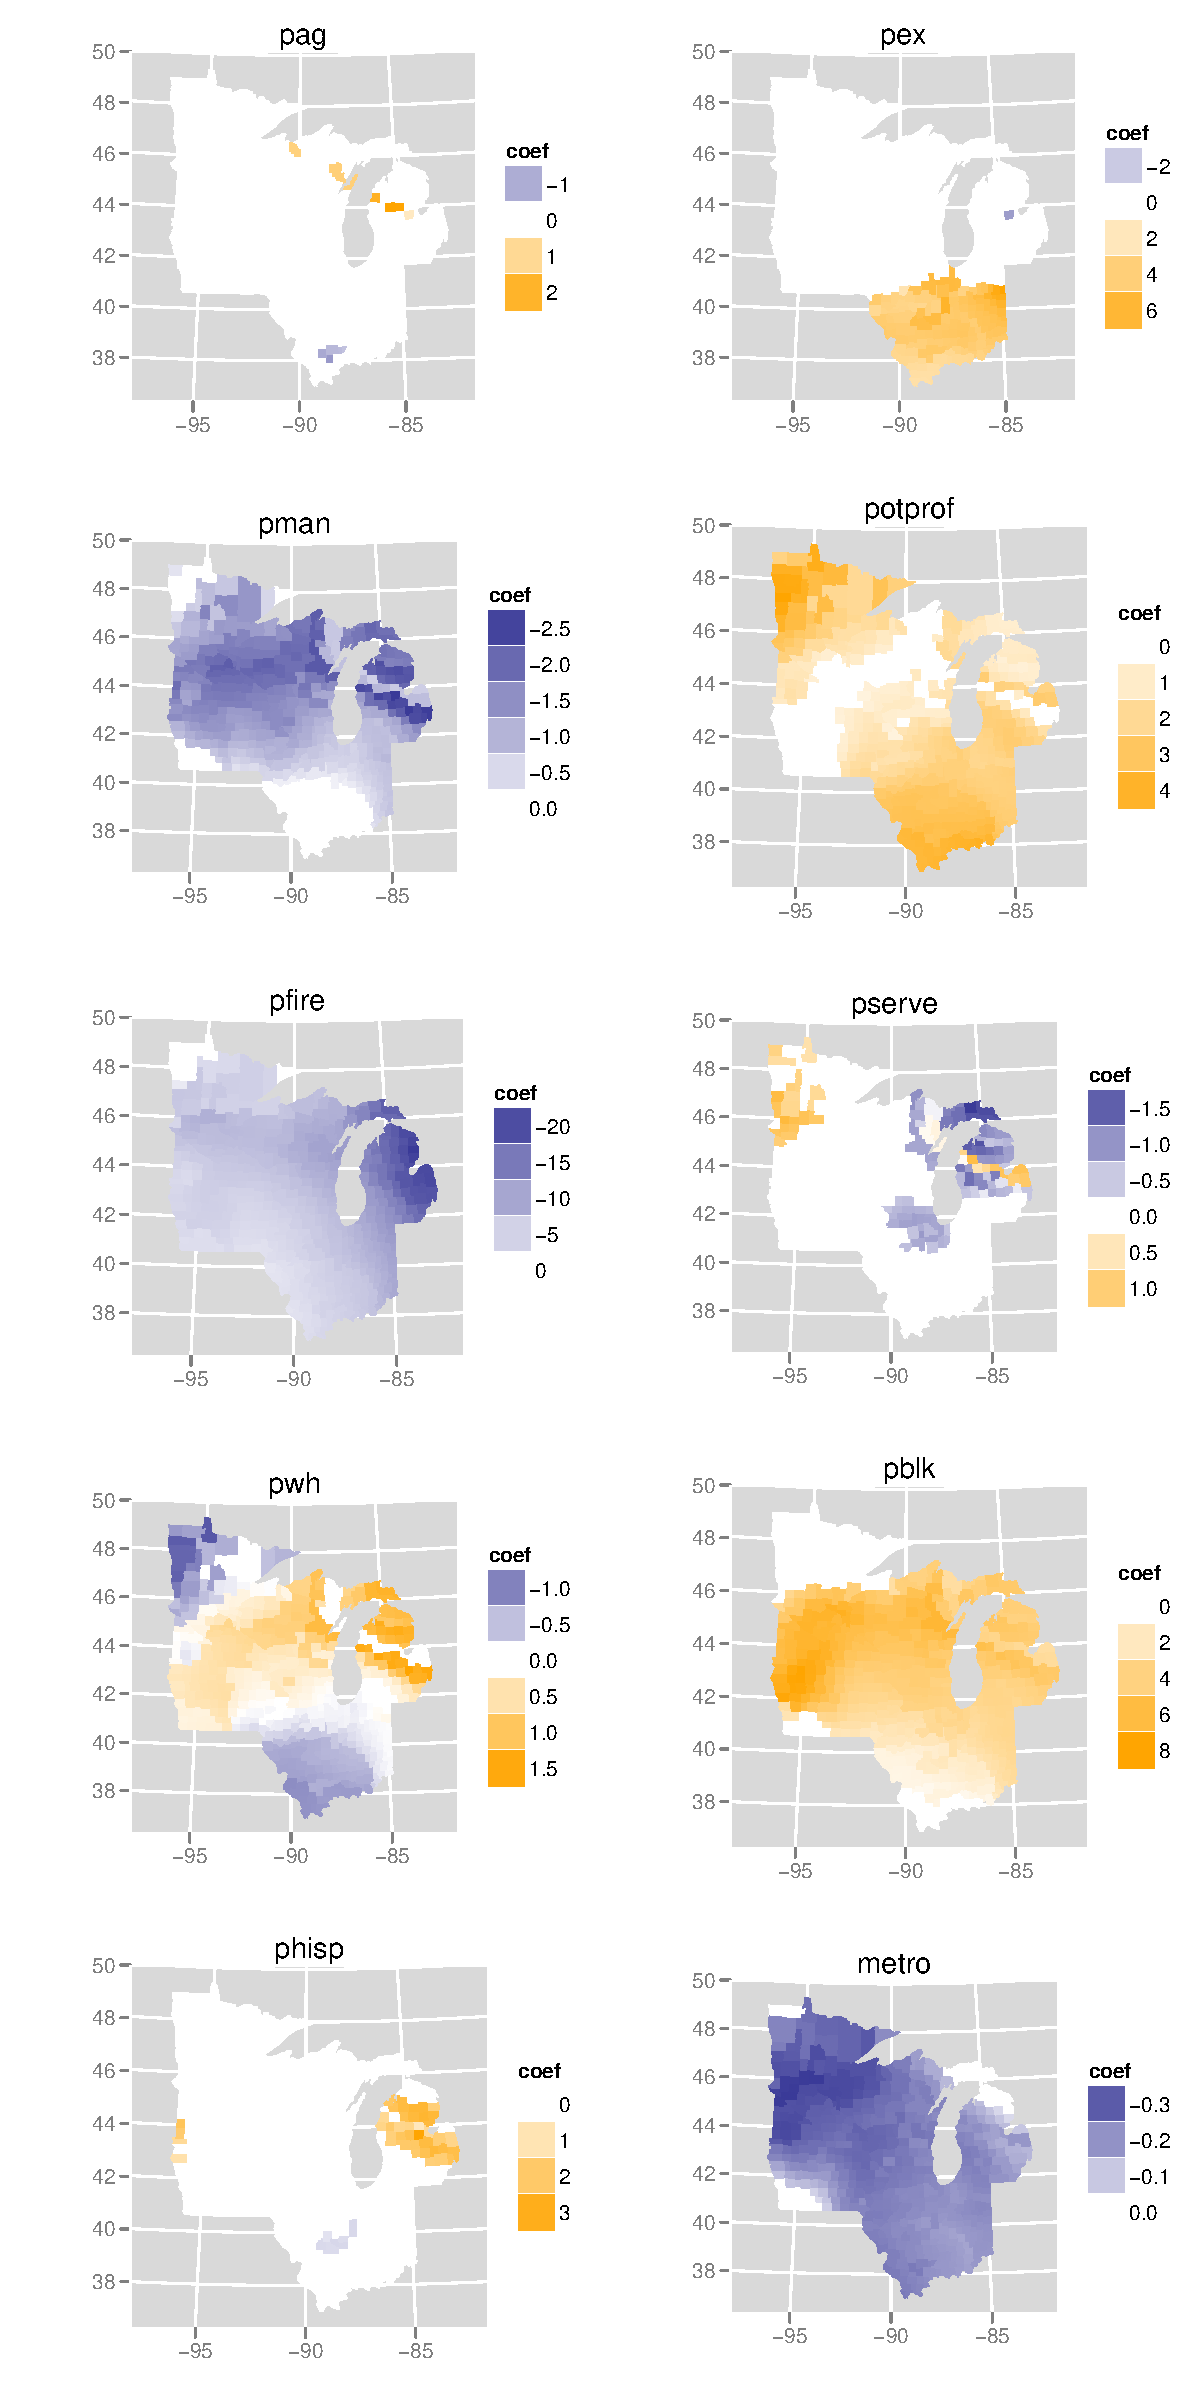
\includegraphics[height=8in]{../../figures/poverty/2000.linear.coefficients.pdf}
			\caption{Estimated coefficient surfaces for the 2000 census.\label{fig:census-coefs-2000}}
		\end{center}
	\end{figure}

	\begin{figure}
		\begin{center}
			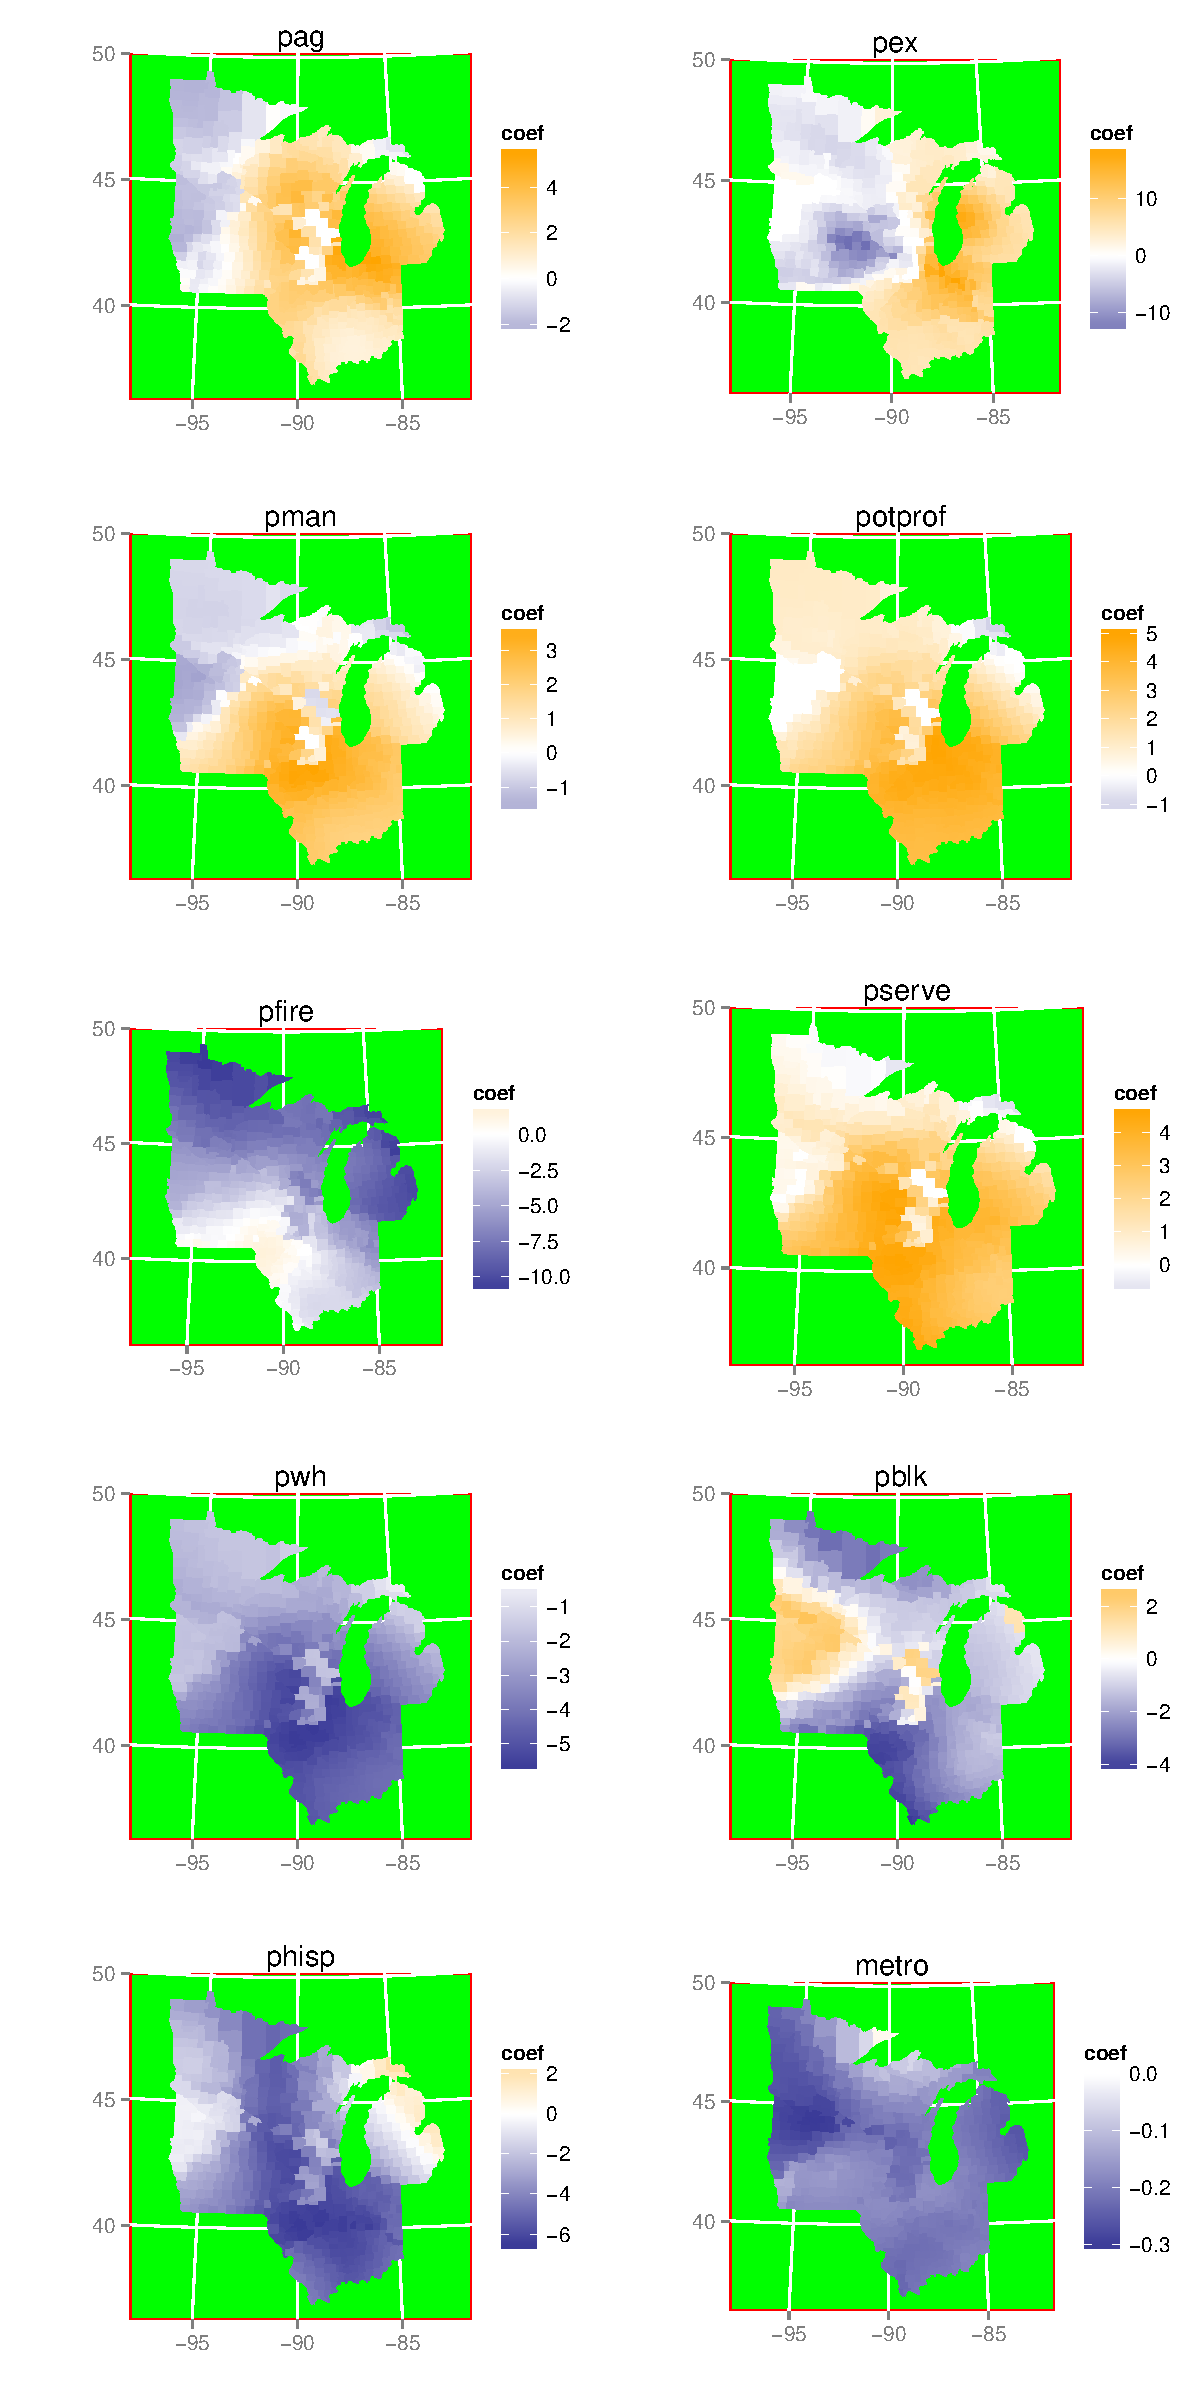
\includegraphics[height=8in]{../../figures/poverty/2006.linear.coefficients.pdf}
			\caption{Estimated coefficient surfaces for the 2006 census.\label{fig:census-coefs-2006}}
		\end{center}
	\end{figure}
	\end{comment}
			
